\chapter[Systèmes d'équations différentielles \life]{Systèmes
 d'équations différentielles d'ordre un\\ \life}\label{ChapSystEquDiff}

\compileTHEO{

Ce chapitre est une très brève introduction aux {\em systèmes d'équations
différentielles d'ordre un}.  Le but principal de cette introduction est de
convaincre le lecteur de l'importance que ces systèmes ont en science
et génie.

Nous présentons une approche qualitative à l'étude des systèmes
d'équations différentielles d'ordre un.  Puisque ces systèmes peuvent
avoir un grand nombre d'inconnues, essayer de les résoudre
analytiquement demanderait une travail énorme et cela en supposant que
c'est possible.  Nous utilisons normalement des méthodes numériques
pour \lgm résoudre\rgm\ les systèmes d'équations différentielles
d'ordre un.  Mais même avec ces méthodes, il est souvent très
difficile d'analyser ces systèmes.  C'est pour cette raison que
l'étude qualitative des systèmes d'équations différentielles d'ordre
un est très importante. 

Nous fournirons une analyse complète dans le cas des systèmes
d'équations différentielles linéaires d'ordre un.  C'est le mieux que
nous puissions faire.  La section sur {\em l'analyse global} nous
fourni des outils pour l'analyse qualitative des
{\em systèmes d'équations différentielles non-linéaire d'ordre un}.
La section sur l'équation de Van der Pol et la section sur le système
prédateurs-proies fournissent deux exemples simples de systèmes
d'équations différentielles non-linéaires d'ordre qui présentent une
dynamique beaucoup plus complexe que celle que nous pouvons observer
pour les systèmes d'équations différentielles linéaires d'ordre un.
L'approche dans ces deux dernières sections est très intuitive et
informelle.  C'est seulement la point de l'iceberg de ce sujet
d'études.

\section{Introduction}

\begin{egg}[][Système prédateurs-proies] \label{PREPRO}
Cet exemple est présent dans la majorité des manuels de mathématiques
pour les sciences biologiques.  Nous nous sommes inspiré de Murray \cite{M}
pour la présentation qui suit.

L'exemple classique d'un système d'équations différentielles d'ordre
un est le système qui décrit le nombre d'individus de deux espèces
animales; une espèce représentant les proies et l'autre représentant
les prédateurs.  Les deux espèces sont en compétition pour leur existence.

Nous pouvons imaginer que, si les prédateurs dévorent trop de proies, ces
prédateurs mettront en danger leur propre existence en détruisant leur source
de nourriture.  Par contre, si le nombre de proies devient très grand, il
sera facile pour les prédateurs de capturer des proies et le nombre de
prédateurs va augmenter.  Qu'arrivera-t-il à long terme? Est-ce que les
espèces vont disparaître?  Est-ce qu'il s'établira un équilibre entre le 
nombre de proies et de prédateurs?

Nous pouvons décrire l'interaction entre les deux espèces à l'aide d'équations
différentielles.  Soit $q(t)$ le nombre de proies au temps $t$ et $p(t)$ le
nombre de prédateurs au temps $t$ dans un espace donné (e.g.\ par
km$^2$).  Le choix des unités pour le temps est déterminé par
l'espérance de vie des proies et prédateurs.  Les unités de temps
normalement utilisées pour les mammifères sont les années.  Pour
certains insectes nous utiliserons les jours.

Lotka et Voltera, deux biomathématiciens à une époque où nous ne
parlions pas de biomathématiques, développèrent séparément (en 1920 et
1926 respectivement) le système d'équations différentielles d'ordre un
suivant.
\begin{equation} \label{LVsyst}
\begin{split}
\dydx{q}{t} &= q(a-b\,p) \\
\dydx{p}{t} &= p(c\,q - d)
\end{split}
\end{equation}
où $a$, $b$, $c$ et $d$ sont des constantes positives.  Ce système
d'équations différentielles porte maintenant le nom de
{\bfseries système (d'équations différentielles) de
Lotka-Voltera}\index{Système de Lotka-Voltera}.

Commençons par expliquer le rôle et la signification des constantes
dans le système (\ref{LVsyst}).  S'il n'y a pas d'interaction entre
les proies et les prédateurs, le nombre de proies et de prédateurs est
décrit par les équations différentielles
\[
\dydx{q}{t} = a\,q \quad \text{et} \quad \dydx{p}{t} = - d\, p \; .
\]
Ces deux équations sont indépendantes et peuvent être résolues par la
méthode de séparation des variables.  La constante $a$ représente le taux
relatif de croissance pour les proies et la constante $-d$ représente le taux
relatif de croissance pour les prédateurs.  Dans ce dernier cas, le taux de
croissance est négatif car les prédateurs vont disparaître par manque de
nourriture si la population de proies est absente.

Nous représentons le nombre de contacts entre les proies et les
prédateurs par le produit $p\,q$.  Ainsi, le terme $-b\,p\,q$ du côté
droit de la première
équation en (\ref{LVsyst}) a un effet négatif sur le taux de croissance des 
proies car $-b\, p \, q \leq 0$.  Par contre le terme $c\,p\,q$ du côté
droit de la deuxième équation en (\ref{LVsyst}) a un effet positif sur le
taux de croissance car $c\,p\,q \geq 0$.  Cela est consistant avec le fait
que lorsqu'un prédateur entre en contact avec une proie, c'est la proie
qui est la grande perdante.

Le système (\ref{LVsyst}) semble dépendre de quatre paramètres: $a$, $b$, $c$
et $d$.  Par contre, il existe une dépendance entre ces quatre paramètres qui
cache la simplicité du système.  Le raisonnement suivant est appelé
{\bfseries non-dimensionalisation}\index{Non-dimensionalisation} et
permet de réduire le nombre de paramètres au nombre minimal de
paramètres nécessaires pour décrire la comportement qualitatif de
(\ref{LVsyst}).

Si nous posons
\[
  q(t) = \frac{d}{c}u(a t) \ , \ p(t) = \frac{a}{b} v(at) \quad
  \text{et} \quad \alpha = \frac{d}{a} ,
\]
nous obtenons
\begin{align*}
q'(t) &= \frac{d}{c}\dfdx{u(at)}{t} = \frac{da}{c}u'(at)
\intertext{et}
p'(t) &= \frac{a}{b}\dfdx{v(at)}{t} = \frac{a^2}{b}v'(at) \ .
\end{align*}
Ainsi, (\ref{LVsyst}) donne
\begin{subequations}  \label{LVsystR}
\begin{align}
\frac{da}{c}u'(at) &= \frac{d}{c}u(a t) \left( a - b \;
\frac{a}{b} v(at) \right) = \frac{ad}{c} u(a t) \left( 1 - v(at) \right)
\label{LVsystRa} \\
\intertext{et}
\frac{a^2}{b}v'(at) &= \frac{a}{b} v(at) \left(
c \; \frac{d}{c}u(a t) - d\right) = \frac{ad}{b} v(at) \left(
u(a t) - 1\right) \ . \label{LVsystRb}
\end{align}
\end{subequations}
Si nous multiplions les deux côtés de (\ref{LVsystRa}) par
$\displaystyle \frac{c}{ad}$ et ceux de (\ref{LVsystRb}) par
$\displaystyle \frac{b}{a^2}$, nous obtenons
\begin{align*}
u'(at) &= u(a t) \left( 1 - v(at) \right) \\
v'(at) &= \frac{d}{a}\; v(at) \left( u(a t) - 1\right) 
= \alpha v(at) \left( u(a t) - 1\right)  \ .
\end{align*}
Finalement, si nous ajustons le temps en posant $\tau = at$, nous obtenons
\begin{equation} \label{ndLVsyst}
\begin{split}
\dydx{u}{\tau} &= u(1-v) \\
\dydx{v}{\tau} &= \alpha \,v(u - 1)
\end{split}
\end{equation}
Qualitativement, (\ref{ndLVsyst}) est équivalant à (\ref{LVsyst});
c'est-à-dire que nous pouvons représenter tous les
{\em types de solutions} que
(\ref{LVsyst}) possède en variant le paramètre $\alpha$ seulement.

Dans ce chapitre, nous développerons des outils pour analyser les systèmes
d'équations différentielles d'ordre comme (\ref{ndLVsyst}).
\end{egg}

\begin{egg}[][Compétition -- exclusion] \label{COMPEXCL}
Comme pour l'exemple précédent, nous nous sommes inspiré de Murray \cite{M}
pour la présentation qui suit.

Le deuxième exemple de systèmes d'équations différentielles d'ordre un
décrit le comportement de deux espèces animales, l'espèce P et
l'espèce Q, restreintes à un même territoire et ayant la même source
de nourriture.

Soit $p(t)$ le nombre d'individus de l'espèce P au temps $t$ et $q(t)$ le
nombre d'individus de l'espèce Q au temps $t$ dans un espace donné.
Comme à l'exemple précédent, le choix des unités pour le temps est
déterminé par l'espérance de vie des deux espèces.

Si les deux espèces occupent des milieux distincts, ils n'entrent donc pas en
compétition pour la nourriture, alors $p$ est gouverné par une équation
logistique et il en est de même pour $q$.  Ce type d'équation a été étudié
au chapitre sur les équations différentielles.  Nous avons
\begin{equation}\label{twoLEQ}
\dydx{p}{t} = a\,p\left(1-\frac{p}{M_p}\right)
\quad \text{et} \quad
\dydx{q}{t} = b\,q\left(1- \frac{q}{M_q}\right) \; .
\end{equation}
La constante $a>0$ est associée au taux de croissance relatif de l'espèce P et
la constante $b>0$ est associée à celui de l'espèce Q.  $M_p$ est le nombre
maximal d'individus de l'espèce P que le milieu peut supporter et $M_q$ est
le nombre maximal d'individus de l'espèce Q que le milieu peut supporter.

Les équations différentielles ci-dessus décrivent la situation où la
consommation de nourriture d'une espèce n'a pas d'effet sur l'autre espèce.
Par contre, si les deux espèces occupent le même milieu, elles entrent en
compétition pour la nourriture disponible.  Pour décrire le nombre
d'individus d'une espèce, il faut donc tenir compte du nombre d'individus de
l'autre espèce.

Nous considérons le système d'équations différentielles d'ordre un suivant.
\begin{subequations} \label{CompExcl}
\begin{align}
\dydx{p}{t} &= a\,p\left(1- \frac{p + c\, q}{M_p} \right) \label{CompExcla} \\
\dydx{q}{t} &= b\,q\left(1- \frac{q + d\, p}{M_q} \right) \label{CompExclb}
\end{align}
\end{subequations}
Les constantes positives $c$ et $d$ sont déterminées par la quantité de
nourriture consommée par chacun des individus des deux espèces -- Peut-être
qu'un individu de l'espèce P a besoin pour survivre du double de la quantité
de nourriture qu'un individu de l'espèce Q a besoin pour survivre.  Les
constantes $c$ et $d$ peuvent aussi dépendre de l'état de la source de
nourriture après le passage d'une espèce -- Peut-être que les individus d'une
espèce détruisent plus de nourriture qu'ils en consomment.

Le terme $(p+c\,q)/M_p$ du côté droit de (\ref{CompExcla}) joue le
même rôle que le terme $p/M_p$ dans l'équation logistique à gauche
dans l'équation (\ref{twoLEQ}).  Il faut tenir compte de l'impact de
l'espèce Q sur la source de nourriture.  Un individu de l'espèce Q a
un effet qui est $c$ fois celle d'un individu de l'espèce P.  De même,
le terme $(q+d\,p)/M_q$ du côté droit de (\ref{CompExclb}) joue le
même rôle que le terme $q/M_q$ dans l'équation logistique à droite
dans l'équation (\ref{twoLEQ}).  Il faut maintenant tenir compte de
l'impact de l'espèce P sur la source de nourriture.  Un individu de
l'espèce P a un effet qui est $d$ fois celle d'un individu de l'espèce
Q.

Le nombre de contacts entre les deux espèces est représenté par le produit
$p\,q$.  Nous parlons de contact lorsque les individus des deux espèces se
nourrissent à la même source.

Le système (\ref{CompExcl}) semble dépendre de six paramètres: $a$, $b$, $c$,
$d$, $M_p$ et $M_q$.  Nous pouvons utiliser la technique de
{\bfseries non-dimensionalisation} pour éliminer certains des
paramètres.

Si nous posons
\begin{align*}
  p(t) &= M_p u(a t) \quad , \quad q(t) = M_q v(a t) \ ,\\
\alpha &= \frac{b}{a} \quad , \quad  \rho = \frac{c\,M_q}{M_p}
\quad \text{et} \quad \xi = \frac{d\,M_p}{M_q} \; .
\end{align*}
et que nous ajustons le temps en posant $\tau = a\,t$, le système
(\ref{CompExcl}) devient le système
\begin{equation} \label{ndCompExcl}
\begin{split}
\dydx{u}{\tau} &= u(1-u - \rho\,v) \\
\dydx{v}{\tau} &= \alpha \,v(1-v-\xi\,u)
\end{split}
\end{equation}
Nous laissons aux lecteurs le soin de vérifier cette conclusion.
Nous avons réduit le nombre de paramètres à trois.  Comme à l'exemple précédent,
(\ref{CompExcl}) et (\ref{ndCompExcl}) sont équivalant
qualitativement.
\end{egg}

\begin{egg}
L'exemple suivant provient en grande partie de Borelli et Coleman \cite{BC}.

Pour qu'un médicament contre le rhume soit efficace, il faut que la quantité
du médicament dans le sang du patient soit plus grande qu'une certaine
valeur minimale pour une période suffisamment longue.

Nous analysons deux médicaments contre le rhume: un décongestionnant et un
antihistaminique.

\noindent{\bfseries Une seule dose}

Le nombre d'unités $x(t)$ d'un médicament dans l'estomac au temps $t$ en
heures satisfait l'équation différentielle 
\begin{equation}\label{dose1}
\dydx{x}{t} = -k_1 x
\end{equation}
et le nombre d'unités $y(t)$ de ce médicament dans le sang au temps $t$ en
heures satisfait l'équation différentielle 
\begin{equation}\label{dose2}
\dydx{y}{t} = k_1 x - k_2 y \; .
\end{equation}
Les constantes $k_1$ et $k_2$ sont positives et déterminées par le médicament
considéré.

$k_1 x(t)$ est le taux d'assimilation du médicament au temps $t$ par le sang
qui traverse l'estomac et $k_2y(t)$ est le taux d'élimination du médicament
au temps $t$ par le foie et les reins.

S'il y a initialement $x(0)=A$ unités du médicament (le patient
avale une dose de $A$ unités) et $y(0)=0$ unité (il n'y a aucune
trace du médicament dans le sang car c'est la première dose que le
patient reçoit), alors la solution de (\ref{dose1}) et (\ref{dose2}) est 
\[
x(t) = A e^{-k_1 t} \quad , \quad
y(t) = -\frac{A k_1 e^{-k_1 t}}{k_1 - k_2}
+ \frac{A k_1 e^{-k_2 t}}{k_1 - k_2} \; .
\]

Pour un décongestionnant, nous estimons que
$k_1 = 1.386$ et $k_2 = 0.1386$.   Supposons que le patient prenne
initialement $A=1$ unité du médicament.  Nous obtenons alors les graphes de
$x$ et $y$ donnés à la figure~\ref{doseFIG1}.

Pour un antihistaminique, nous estimons que $k_1=0.6931$ et
$k_2=0.0231$.  Supposons encore que le patient prenne
initialement $A=1$ unité du médicament.  Nous obtenons les graphes de
$x$ et $y$ donnés à la figure~\ref{doseFIG2}.

\begin{figure}
\centering
\subfloat[décongestionnant]{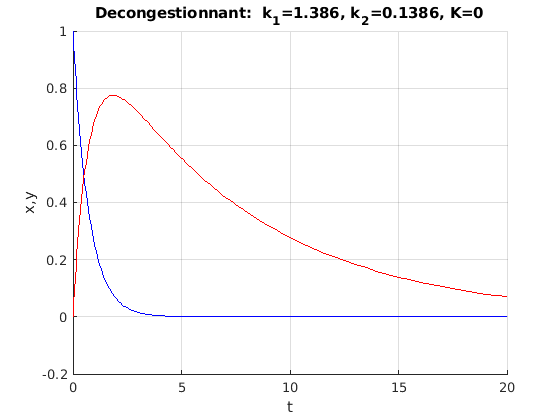
\includegraphics[width=7cm]{18_syst_equ_diff/drug1a_dec}\label{doseFIG1}}
\qquad
\subfloat[antihistaminique]{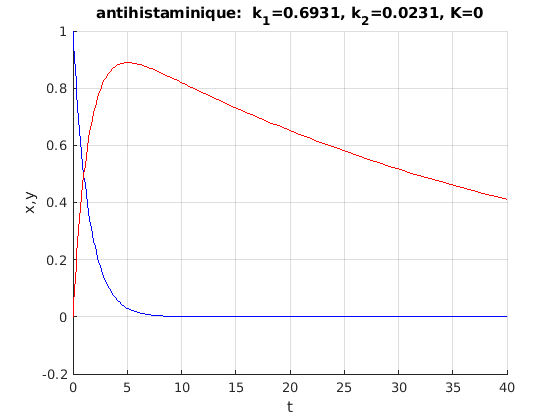
\includegraphics[width=7cm]{18_syst_equ_diff/drug1a_ant}\label{doseFIG2}}
\caption[Graphes de la quantité de décongestionnant et
d'antihistaminique dans l'estomac et dans le sang pour une seule dose]
{(a) Graphes de la quantité de décongestionnant dans l'estomac (en
bleu) et dans le sang (en rouge) pour une seule dose.
(b) Graphes de la quantité d'antihistaminique dans l'estomac (en
bleu) et dans le sang (en rouge) pour une seule dose.}\label{doseFIG12}
\end{figure}

% \MATHfig{18_syst_equ_diff/drug1a_dec}{8cm}{Graphes de la quantité de
% décongestionnant dans l'estomac et dans le sang pour une seule
% dose}{Graphes de la quantité de décongestionnant dans l'estomac (en
% bleu) et dans le sang (en rouge) pour une seule dose.}{doseFIG1} 

% \MATHfig{18_syst_equ_diff/drug1a_ant}{8cm}{Graphes de la quantité
% d'antihistaminique dans l'estomac et dans le sang pour une seule
% dose}{Graphes de la quantité d'antihistaminique dans l'estomac (en
% bleu) et dans le sang (en rouge) pour une seule dose.}{doseFIG2}

Si seulement les quantités de médicament dans le sang sont considérées,
l'antihistaminique semble avoir un plus long effet.  Par contre, le
décongestionnant semble agir plus rapidement.

\noindent{\bfseries Un médicament administré de façon continue}

Certaines pilules sont formées d'un très grand nombre de petites boules qui se
dissolvent dans l'estomac à des rythmes différents.  Le résultat est que le
médicament n'est pas absorbé par l'estomac d'un seul coup comme dans le cas
précédent mais il est absorbé par l'estomac à un taux constant de $K$
unités par heure (pour la durée de la pilule).

Supposons que la fréquence à laquelle le patient prend une pilule soit
telle que le taux d'absorption dans l'estomac soit constant à $K$ unités par
heure, alors le nombre d'unités $x(t)$ dans l'estomac au temps $t$ en heures
et le nombre d'unités $y(t)$ dans le sang au temps $t$ en heures sont
gouvernés par les équations différentielles
\begin{equation} \label{dose3}
\begin{split}
\dydx{x}{t} &= K -k_1 x \\
\dydx{y}{t} &= k_1 x - k_2 y
\end{split} \ .
\end{equation}

Dans le présent problème, nous avons $x(0)=0$ et $y(0)=0$ unité
initialement.  La condition $x(0)=0$ ne veut pas dire que le patient
ne prend pas de médicament.  Le patient reçoit une dose de $K$ unités par
heure.  La condition $x(0)=0$ veut dire que le patient n'a pas de
médicament dans l'estomac au départ.  De même, $y(0)=0$ veut dire que
le patient n'a pas de médicament dans le sang au départ.

La solution de (\ref{dose3}) est
\begin{align*}
x(t) &= -\frac{K\left(-1 + e^{-k_1 t}\right)}{k_1} \\
y(t) &= -\frac{K\left(-k_1 + k_2 - k_2 e^{-k_1 t} + k_1 e^{-k_2
      t}\right)}{k_2 (k_1 - k_2)}
\end{align*}

La quantité $x(t)$ du médicament dans l'estomac converge vers
$x = K/k_1$ lorsque $t$ tend vers l'infini (de plus,
$x'(t) \rightarrow 0$ lorsque $t \rightarrow \infty$) et la quantité $y(t)$
du médicament dans le sang converge vers $y = K/k_2$ lorsque $t$
tend vers plus l'infini (de plus, $y'(t) \rightarrow 0$ lorsque
$t \rightarrow \infty$).

Utilisons les valeurs $k_1 = 1.386$ et $k_2 = 0.1386$ pour un
décongestionnant qui ont été données précédemment et supposons que
$K=1$ unité par heure.  Nous obtenons alors les graphes de $x$ et $y$ donnés
à la figure~\ref{doseFIG3}.

Utilisons les valeurs $k_1=0.6931$ et $k_2=0.0231$ pour un
antihistaminique qui ont été données précédemment et supposons
toujours que $K=1$ unité par heure.  Nous obtenons alors les graphes de $x$
et $y$ donnés à la figure~\ref{doseFIG4}.

\begin{figure}
\centering
\subfloat[décongestionnant]{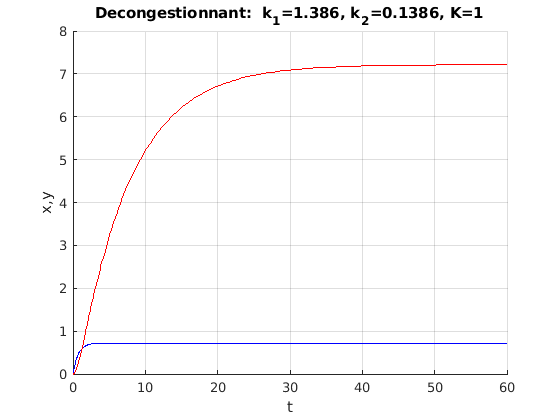
\includegraphics[width=7cm]{18_syst_equ_diff/drug1b_dec}\label{doseFIG3}}
\qquad
\subfloat[antihistaminique]{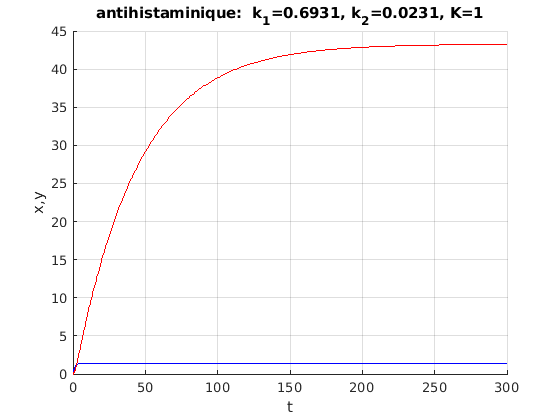
\includegraphics[width=7cm]{18_syst_equ_diff/drug1b_ant}\label{doseFIG4}}
\caption[Graphes de la quantité de décongestionnant et
d'antihistaminique dans l'estomac et dans le sang pour une médication
administré de façon continue]
{(a) Graphes de la quantité de décongestionnant dans l'estomac (en
bleu) et dans le sang (en rouge) pour une médication administré de
façon continue.
(b) Graphes de la quantité d'antihistaminique dans l'estomac (en
bleu) et dans le sang (en rouge) pour une médication administré de
façon continue.}\label{doseFIG34}
\end{figure}

% \MATHfig{18_syst_equ_diff/drug1b_dec}{8cm}{Graphes de la quantité de
% décongestionnant dans l'estomac et dans le sang pour une médication
% administré de continue}{Graphes de la quantité de décongestionnant
% dans l'estomac (en bleu) et dans le sang (en rouge) pour une
% médication administré de façon continue.}{doseFIG3}

% \MATHfig{18_syst_equ_diff/drug1b_ant}{8cm}{Graphes de la quantité
% d'antihistaminique dans l'estomac et dans le sang pour une
% médication administré de façon continue}{Graphes de la quantité
% d'antihistaminique dans l'estomac (en bleu) et dans le sang (en rouge)
% pour une médication administré de façon continue.}{doseFIG4}

Le décongestionnant et l'antihistaminique ont des comportements semblables à
long terme dans le présent cas.  $x'(t) \rightarrow 0$ et
$y'(t) \rightarrow 0$ lorsque $t \rightarrow \infty$.  Plus précisément,
$x(t)$ est asymptotique à $x = K/k_1$ et $y(t)$ est asymptotique à
$x = K/k_2$ lorsque $t \rightarrow \infty$.  Si seulement les 
quantités de médicament dans le sang sont considérées, le
décongestionnant commence à agir beaucoup plus rapidement que
l'antihistaminique.  Par contre, l'action de l'antihistaminique est
beaucoup plus forte.

\noindent{\bfseries Un médicament administré à intervalle régulier}

Dans l'exemple précédent, nous avons supposé que le médicament est
absorbé par l'estomac à un taux constant de $K$ unités par heure (pour
la durée de la pilule) et que le patient prend une pilule à intervalle
régulier de façon à maintenir le taux d'absorption constant à $K$
unités par heure.  C'est une situation idéale qui est presque
impossible à satisfaire.

La situation suivante est plus réaliste.  Supposons que le type de pilules
utilisée soit celui de la section précédente.  Plus précisément,
supposons que le médicament entre dans l'estomac à un taux constant de
$K=12$ unités par heure durant une demi-heure.  Après une demi-heure,
la pilule a été complètement assimilée par l'organisme et il n'y a
plus de médicament qui entre dans l'estomac.  De plus, supposons
que le patient prend une pilule à toutes les six heures.

Le taux d'absorption par l'estomac du médicament est décrit par la formule
\[
F(t) = \sum_{n=0}^N K (H(t + 6 n) - H(t - 0.5 + 6 n))
\]
où $H$ est la fonction de Heaviside définie par
\[
H(t) = \begin{cases}
0 & \qquad \text{si} \quad t<0 \\
1 & \qquad \text{si} \quad t\geq 0
\end{cases}
\]
et $N+1$ est le nombre de pilules prisent par le patient.  Le graphe
de $F$ pour les quatre premières pilules (i.e.\ $N=3$) est donné à la
figure~\ref{doseFIG5}.  C'est ce que nous appelons une onde carrée.

\MATHfig{18_syst_equ_diff/step_funct}{8cm}{Le taux d'absorption
d'un médicament pris à intervalles réguliers}{Le taux d'absorption
d'un médicament pris à intervalles réguliers.}{doseFIG5}

Dans ce cas, le nombre d'unités $x(t)$ dans l'estomac au temps $t$ en heures
et le nombre d'unités $y(t)$ dans le sang au temps $t$ en heures sont
gouvernés par les équations
\begin{equation} \label{dose4}
\begin{split}
\dydx{x}{t}(t) &= -k_1 x(t) + F(t) \\
\dydx{y}{t}(t) &= k_1 x(t) - k_2 y(t)
\end{split}
\end{equation}

Reprenons les deux types de médicament qui ont été considérés
précédemment; à savoir le décongestionnant et l'antihistaminique.

Remarquons que la première équation de (\ref{dose4}) est indépendante de la
fonction $y$.  Cette équation peut donc être résolue à l'aide des
{\em transformations de Laplace}; c'est un des sujets d'un premier
cours d'équations différentielles.  Après avoir trouvé $x$, la
deuxième équation de (\ref{dose4}) devient une équation linéaire
d'ordre un pour la fonction $y$.  Nous pourrions (avec amplement
de temps et de patience, ou avec un logiciel de calculs symboliques)
trouver une expression pour $x$ et $y$. Puisque nous voulons tracer le
graphe des solutions $x$ et $y$ de (\ref{dose4}), au lieu de trouver
une expression pour $x$ et $y$, nous résolvons numériquement le système
(\ref{dose4}).  Il faut porter une attention particulière aux points
où le côté droit de l'équation (\ref{dose4}) est discontinu.

Comme dans le cas de la médication continue, nous supposons que
$x(0)=0$ unité et $y(0)=0$ unité.

Pour le décongestionnant, nous avons $k_1=1.386$ et $k_2=0.1386$.  Les
graphes de $x$ et $y$ sont donnés à la figure~\ref{doseFIG6}.

Les graphes à la figure~\ref{doseFIG6} suggèrent que la quantité de
médication dans l'estomac a un comportement périodique et ne dépassera pas
environ $4.5$ unités.  De plus, la quantité de médication dans le sang semble
tendre vers une fonction périodique de moyenne $7$ unités et d'amplitude
environ $1.8$  Nous supposons ici que le patient ne cesse pas de prendre des
pilules et donc $N$ augmente.  Est-ce que le patient risque d'avoir une
surdose du médicament?  Une analyse mathématique plus poussée est
nécessaire pour montrer que le patient ne souffrira pas d'une surdose.

Nous traçons le graphe de la quantité d'antihistaminique pour $k_1=0.6931$
et $k_2=0.0231$ dans l'estomac et dans le sang en fonction du temps à la
figure~\ref{doseFIG7}.  Nous supposons toujours que $x(0)=0$ unité et $y(0)=0$
unité.

\begin{figure}
\centering
\subfloat[décongestionnant]{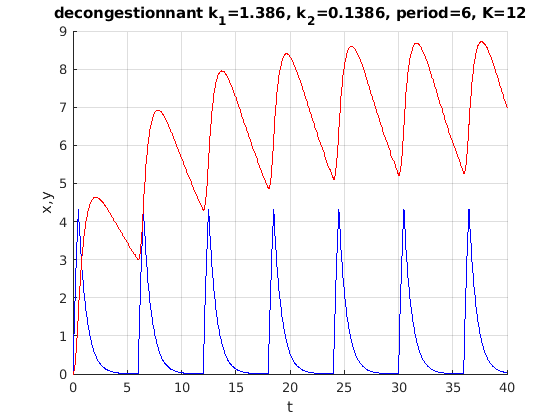
\includegraphics[width=7cm]{18_syst_equ_diff/drug2a_dec}\label{doseFIG6}}
\qquad
\subfloat[antihistaminique]{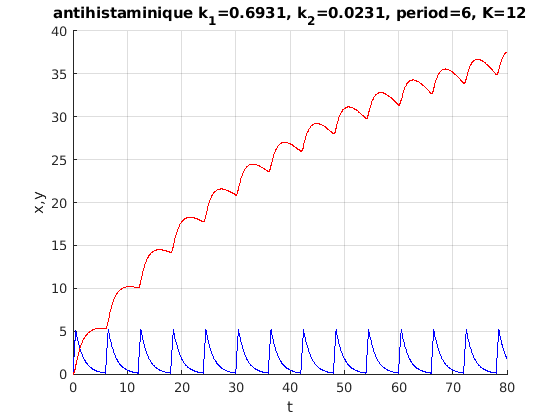
\includegraphics[width=7cm]{18_syst_equ_diff/drug2a_ant}\label{doseFIG7}}
\caption[Graphes de la quantité de décongestionnant et
d'antihistaminique dans l'estomac et dans le sang pour une médication
administré à intervalles réguliers]
{(a) Graphes de la quantité de décongestionnant dans l'estomac (en
bleu) et dans le sang (en rouge) pour une médication administré à
intervalles réguliers.
(b) Graphes de la quantité d'antihistaminique dans l'estomac (en
bleu) et dans le sang (en rouge) pour une médication administré à
intervalles réguliers.}\label{doseFIG67}
\end{figure}

% \MATHfig{18_syst_equ_diff/drug2a_dec}{8cm}{Graphes de la quantité de
% décongestionnant dans l'estomac et dans le sang pour une médication
% administrée à intervalles réguliers}{Graphes de la quantité de
% décongestionnant dans l'estomac (en bleu) et dans le sang
% (en rouge) pour une médication administrée à intervalles
% réguliers.}{doseFIG6}

% \MATHfig{18_syst_equ_diff/drug2a_ant}{8cm}{Graphes de la quantité
% d'antihistaminique dans l'estomac et dans le sang pour une médication
% administrée à intervalles réguliers}{Graphes de la quantité
% d'antihistaminique dans l'estomac (en bleu) et dans le sang (en rouge)
% pour une médication administrée à intervalles réguliers.}{doseFIG7}

Comme dans le cas du décongestionnant, le graphe de la quantité
d'antihistaminique dans l'estomac en fonction du temps suggèrent que la
quantité de médication dans l'estomac a un comportement périodique et ne
dépassera pas environ $5$ unités.  Par contre, la quantité
d'antihistaminique dans le sang semble en moyenne augmenter sans borne
supérieure.  En fait, une étude plus poussée montre que la quantité
d'antihistaminique dans le sang approche une fonction périodique de moyenne
environ $43$ unités et de période environ $1$.  Dépendant des unités
utilisées, nous risquons d'intoxiquer le patient car la quantité
d'antihistaminique dans le sang devient en moyenne $11$ fois la
quantité dans l'estomac.
\end{egg}

\section{Énoncé du problème général}

La forme générale d'un {\bfseries système d'équations différentielles
d'ordre un}\index{Système d'équations différentielles!d'ordre un} dans
$\RR^2$ est
\begin{equation} \label{sediff1}
\begin{split}
\dydx{x_1}{t} &= f_1(t,x_1,x_2) \\
\dydx{x_2}{t} &= f_2(t,x_1,x_2)
\end{split}
\end{equation}
où $f_i:]a,b[\times \RR^2 \rightarrow \RR$ pour $i=1$ et $2$.

La majorité des définitions et résultats que nous allons énoncés ont un
équivalent pour les systèmes d'équations différentielles d'ordre un
qui ont plus de deux inconnus et deux équations différentielles.  Nous
allons nous limiter aux systèmes composés de deux inconnus et deux
équations différentielles.

Si $f_1$ et $f_2$ ne dépendent pas de $t$, nous obtenons le
{\bfseries système d'équations différentielles autonomes
d'ordre un}\index{Système d'équations différentielles!autonome}
\begin{equation} \label{sediff2}
\begin{split}
\dydx{x_1}{t} &= f_1(x_1,x_2) \\
\dydx{x_2}{t} &= f_2(x_1,x_2)
\end{split}
\end{equation}
où $f_i:\RR^2 \rightarrow \RR$ pour $i=1$ et $2$.  C'est ce genre de
systèmes d'équations différentielles que nous considérons dans ce
chapitre.  Une forme brève pour (\ref{sediff2}) est
\begin{equation} \label{sediff3}
\dydx{\VEC{x}}{t} = \VEC{f}(\VEC{x})
\end{equation}
où
\[
\VEC{x} = \begin{pmatrix} x_1 \\ x_2 \end{pmatrix}
\quad , \quad
\dydx{\VEC{x}}{t} =
\begin{pmatrix} \displaystyle \dydx{x_1}{t} \\[1em]
\displaystyle \dydx{x_2}{t} \end{pmatrix}
\quad \text{et} \quad
\VEC{f}(\VEC{x}) = \begin{pmatrix} f_1(x_1,x_2)\\
f_2(x_1,x_2)
\end{pmatrix} \; .
\]

Le but est de trouver $2$ fonctions, $\phi_1:]a,b[ \rightarrow \RR$ et
$\phi_2:]a,b[ \rightarrow \RR$, telles que si nous remplaçons $x_1$ par
$\phi_1$ et $x_2$ par $\phi_2$ dans (\ref{sediff2}) alors l'équation
est satisfaite pour tout $t \in ]a,b[$.

\begin{defn} \index{Système d'équations différentielles!solution}
Une fonction
\begin{align*}
\phi:]a,b[ & \rightarrow \RR^2 \\
t &\mapsto
\begin{pmatrix}
\phi_1(t) \\ \phi_2(t)
\end{pmatrix}
\end{align*}
est une {\bfseries solution} du système d'équations différentielles
(\ref{sediff2}) si
\[
\begin{split}
\dydx{\phi_1}{t}(t) &= f_1(\phi_1(t),\phi_2(t)) \\
\dydx{\phi_2}{t}(t) &= f_2(\phi_1(t),\phi_2(t))
\end{split}
\]
pour tout $t \in]a,b[$.
\end{defn}

\begin{egg}
Soit le système d'équations différentielles autonome d'ordre un
\begin{equation}\label{systdfes1}
\begin{split}
\dydx{x_1}{t} &= x_1 + 2\,x_2\\
\dydx{x_2}{t} &= 5\,x_1 - 2\,x_2
\end{split}
\end{equation}
Les fonctions $\phi_1(t) = e^{3t}-2\,e^{-4t}$ et
$\phi_2(t) = e^{3t}+5\,e^{-4t}$ satisfont (\ref{systdfes1}) car
\begin{align*}
\dydx{\phi_1}{t}(t) &= \dfdx{\left(e^{3t}-2\,e^{-4t}\right)}{t}
= 3\,e^{3t}+8\,e^{-4t} \\
&= \left(e^{3t}-2\,e^{-4t}\right) +2\left(e^{3t}+5\,e^{-4t}\right)
= \phi_1(t) + 2\,\phi_2(t)
\end{align*}
et
\begin{align*}
\dydx{\phi_2}{t}(t) &= \dfdx{\left(e^{3t}+5\,e^{-4t}\right)}{t}
= 3\,e^{3t}-20\,e^{-4t} \\
&= 5\left(e^{3t}-2\,e^{-4t}\right) -2\left(e^{3t}+5\,e^{-4t}\right)
= 5\phi_1(t) - 2\,\phi_2(t)
\end{align*}
pour tout $t$.  Nous verrons prochainement comment trouver $\phi_1$ et
$\phi_2$ pour un système d'équations différentielles de la forme
(\ref{systdfes1}).

Les fonctions $\phi_1$ et $\phi_2$ donne la solution
\[
\phi(t) =
\begin{pmatrix}
\phi_1(t) \\
\phi_2(t)
\end{pmatrix}
=
\begin{pmatrix}
e^{3t}-2\,e^{-4t} \\ e^{3t}+5\,e^{-4t}
\end{pmatrix}
= e^{3t} \begin{pmatrix} 1 \\ 1 \end{pmatrix}
+ e^{-4t} \begin{pmatrix} -2 \\ 5 \end{pmatrix}
\]
de (\ref{systdfes1}).
\label{syst_egg0}
\end{egg}

Il est commun d'imposer une {\bfseries condition initiale}\index{Système
d'équations différentielles!condition initiale} au système d'équations
différentielles (\ref{sediff2}).  C'est-à-dire, de demander que la solution
$\phi:]a,b[\rightarrow \RR^2$ de (\ref{sediff2}) satisfasse
\[
  \phi(t_0) = \begin{pmatrix} \phi_1(t_0) \\ \phi_2(t_0) \end{pmatrix}
  = \begin{pmatrix} x_{0,1} \\ x_{0,2} \end{pmatrix}
\]
pour $t_0\in]a,b[$ et
$\displaystyle \VEC{x}_0 = \begin{pmatrix} x_{0,1} \\ x_{0,2} \end{pmatrix}$
donnés.

\begin{egg}
Nous invitons les lecteurs à vérifier que
\[
\phi(t) = a_1 \, e^{3t} \begin{pmatrix} 1 \\ 1 \end{pmatrix}
+ a_2\, e^{-4t} \begin{pmatrix} -2 \\ 5 \end{pmatrix}
\]
est une solution du système d'équations différentielles
(\ref{systdfes1}) de l'exemple~\ref{syst_egg0} quelles que soit les
valeurs données aux constantes $a_1$ et $a_2$.

Pour trouver la solution de (\ref{systdfes1}) qui satisfasse la
condition initiale
\begin{equation}
\phi(0)= \begin{pmatrix} 4 \\ -3 \end{pmatrix}  \ , \label{sedlin_init}
\end{equation}
il faut déterminer $a_1$ et $a_2$ tels que
\[
\phi(0) = a_1 \, \begin{pmatrix} 1 \\ 1 \end{pmatrix}
+ a_2\,\begin{pmatrix} -2 \\ 5 \end{pmatrix}
= \begin{pmatrix} a_1-2\,a_2 \\ a_1 + 5\,a_2 \end{pmatrix}
= \begin{pmatrix} 4 \\ -3 \end{pmatrix}  \; .
\]
Si nous résolvons le système d'équations linéaires
$a_1-2\,a_2 = 4$ et $a_1+5\,a_2 = -3$, nous trouvons $a_1=2$ et $a_2=-1$.
La solution du système (\ref{systdfes1}) qui satisfait la condition
initiale (\ref{sedlin_init}) est
\[
\phi(t) = 2 \, e^{3t} \begin{pmatrix} 1 \\ 1 \end{pmatrix}
- \, e^{-4t} \begin{pmatrix} -2 \\ 5 \end{pmatrix}
= \begin{pmatrix} 2 \, e^{3t} + 2\, e^{-4t} \\
2 \, e^{3t} -5 \, e^{-4t}
\end{pmatrix} \; .
\]
Nous parlons de \lgm la solution\rgm.  Pourrions-nous avoir une autre
fonction $\phi$ qui satisfait ce système d'équations différentielles
et la condition initiale?  Nous donnerons prochainement des conditions
sur le système d'équations différentielles qui assurent l'existence et
l'unicité d'une solution.
\label{syst_egg1}
\end{egg}

\begin{defn} \index{Système d'équations différentielles!orbite}
{\bfseries L'orbite} d'une solution $\phi:]a,b[\rightarrow \RR^2$ de
(\ref{sediff2}) est l'image
\[
\{ \phi(t) :  a < t < b \}
\]
de cette solution dans le plan.  L'orbite est une courbe dans le plan.
Le {\bfseries portrait de phases} de (\ref{sediff2}) est l'ensemble
des orbites.
\end{defn}

\begin{egg}
L'orbite de la solution 
\[
\phi(t) =
\begin{pmatrix}
2 e^{3t}+ 2\,e^{-4t} \\ 2 e^{3t} - 5\,e^{-4t}
\end{pmatrix}
\]
de l'exemple~\ref{syst_egg1} est la courbe avec une flèche représentée
à la figure~\ref{LINSYST1}.
\end{egg}

\PDFfig{18_syst_equ_diff/lin_syst1}{L'image d'une solution
$\phi:\RR\rightarrow \RR^2$ définie une courbe dans le plan}{L'orbite
de la solution $\phi:\RR\rightarrow \RR^2$ de l'équation différentielle de
l'exemple~\ref{syst_egg1}.  La flèche indique le déplacement le long
de l'orbite lorsque $t$ augmente.}{LINSYST1}

Puisque nous allons généralement étudier les systèmes d'équations
différentielles de la forme (\ref{sediff2}) où $f_1$ et $f_2$ sont
différentiable, le théorème suivant nous assure qu'il y aura toujours
une et une seule solution associée à une condition initiale.

\begin{theorem}
Si les fonctions $f_1:\RR^2 \rightarrow \RR$ et $f_2:\RR^2\rightarrow \RR$
qui décrivent le système d'équation différentielles
(\ref{sediff2}) sont différentiables, alors il existe une et une seule 
solution $\phi$ de (\ref{sediff2}) qui satisfait la condition initiale
$\phi(0) = \VEC{x}_0 \in \RR^2$.
\end{theorem}

\begin{rmk}
Puisqu'il y a une et une seule solution de (\ref{sediff2}) qui passe par un
point donné (i.e.\ qui satisfait une condition initiale donnée), les orbites
ne se coupent pas.
\end{rmk}

Il est généralement très difficile de résoudre les systèmes d'équations
différentielles.  Très souvent, nous ne sommes pas directement intéressés aux
solutions du système d'équations différentielles mais simplement à leur
comportement lorsque nous progressons dans le temps. Qu'arrive-t-il aux
solutions lorsque nous regardons très loin dans le temps?

\section{Systèmes d'équations différentielles linéaires d'or\-dre un}

Nous débutons notre étude des systèmes d'équations différentielles
d'ordre un par l'étude d'une classe de systèmes qui sont \lgm très
simples\rgm\ à analyser.  Il ne faut pas en conclure que ces systèmes
n'auront pas d'importance par la suite.  C'est tout à fait le
contraire.  Ils joueront un rôle primordial dans l'analyse de systèmes
d'équations différentielles beaucoup plus compliqués. Les résultats de
la présente section et leur généralisation à $\RR^n$ sont des outils
très fréquemment utilisés par les chercheurs en biomathématiques.

Un {\bfseries système d'équations différentielles linéaires d'ordre
un}\index{Système d'équations différentielles!linéaires} dans
$\RR^2$ est un système d'équations différentielles de la forme
\begin{align*}
\dydx{x_1}{t} &= a\,x_1 + b\, x_2 \\
\dydx{x_2}{t} &= x\,x_1 + d\, x_2
\end{align*}
où $a$, $b$, $c$ et $d$ sont des constantes.  Si nous posons
\[
A = \begin{pmatrix} a & b \\ c & d \end{pmatrix} \ ,
\]
nous pouvons récrire le système d'équations différentielles précédent sous la
forme
\begin{equation} \label{linclass}
\dydx{\VEC{x}}{t} = A \VEC{x}
\end{equation}
où
\[
\VEC{x} = \begin{pmatrix} x_1 \\ x_2 \end{pmatrix}
\quad \text{et} \quad
\dydx{\VEC{x}}{t} = 
\begin{pmatrix} \displaystyle \dydx{x_1}{t} \\[2ex]
\displaystyle \dydx{x_2}{t} \end{pmatrix} \; .
\]

Nos connaissances sur les valeurs et vecteurs propres vont nous
permettre de résoudre les systèmes d'équations différentielles
linéaires d'ordre un.  En fait, les solutions possibles de
(\ref{linclass}), et donc les portraits de phases pour
(\ref{linclass}), peuvent être groupés en un petit nombre de classes
selon le signe des valeurs propres de $A$ et le nombre de vecteurs
propres non colinéaires.  Nous résumons les résultats dans les trois
propositions suivantes.

\begin{prop}
Si la matrice $A$ de l'équation (\ref{linclass}) possède deux valeurs
propres réelles $\lambda_1$ et $\lambda_2$ distinctes, nous choisissons
$\VEC{v}_1$ un vecteur propre associé à $\lambda_1$ et $\VEC{v}_2$ un
vecteur propre associé à $\lambda_2$.  Les solutions de
(\ref{linclass}) sont de la forme
\begin{equation}\label{gsOFls1}
\VEC{x}(t)= a_1\,e^{\lambda_1\,t} \VEC{v}_1 + a_2\,e^{\lambda_2\,t}
\VEC{v}_2
\end{equation}
où $a_1$ et $a_2$ sont des constantes.  Nous retrouvons à la
figure~\ref{LINEARA3} les portraits de phases possibles dans cette
situation.
\end{prop}

\PDFfig{18_syst_equ_diff/linearA3}{Des portraits de phases possibles
pour un système d'équation différentielles linéaires d'ordre un dans $\RR^2$ si
les valeurs propres sont réelles et distinctes.}{Des portraits de
phases possibles pour (\ref{linclass}) si les valeurs propres sont
réelles et distinctes.}{LINEARA3}

\begin{prop}
Si la matrice $A$ de l'équation (\ref{linclass}) possède une seule
valeur propre $\lambda$, il y a deux cas possibles.  S'ils existent deux
vecteurs propres $\VEC{v}_1$ et $\VEC{v}_2$ associés à $\lambda$ qui
ne sont pas colinéaires, alors la solution est donnée par
(\ref{gsOFls1}).  Si ce n'est pas le cas, les vecteurs propres
associés à $\lambda$ sont donc tous colinéaires, alors les solutions de
(\ref{linclass}) sont de la forme
\[
\VEC{x}(t)= a_1\,e^{\lambda\,t} \VEC{v} + a_2\,e^{\lambda\,t}
\left( \VEC{u} + t \VEC{v} \right)
\]
où $a_1$ et $a_2$ sont des constantes, $\VEC{v}$ un vecteur propre
associé à $\lambda$ et $\VEC{u}$ est une solution de
$(A-\lambda\,\Id)\VEC{u} = \VEC{v}$.
Nous retrouvons à la figure~\ref{LINEARA5} un portrait de phases possible
dans ce dernier cas.  Les solutions approchent de l'origine lorsque
$\lambda<0$ et s'éloignent de l'origine lorsque $\lambda>0$.
\end{prop}

\PDFfig{18_syst_equ_diff/linearA5}{Un portrait de phases possible
pour un système d'équation différentielles linéaires d'ordre un dans
$\RR^2$ s'il n'y a qu'une valeur propre réelle et tous les vecteur
propres sont colinéaires}{Un portrait de phases possible pour
(\ref{linclass}) s'il n'y a qu'une valeur propre réelle et tous les
vecteur propres sont colinéaires.}{LINEARA5}

\begin{prop} \label{COLsolution}
Si la matrice $A$ de l'équation (\ref{linclass}) possède une paire de
vecteurs propres complexes $\lambda_1$ et $\lambda_2$, alors
$\lambda_1 = \overline{\lambda}_2$ puisque les composantes de la
matrice $A$ sont réelles.  Supposons que $\lambda_1 = \alpha + i\beta$
avec $\beta \neq 0$.  Soit $\VEC{v}_1 = \VEC{u}_1 + i \VEC{u}_2$, avec
$\VEC{u}_i \in \RR^2$, un vecteur propre associé à la valeur propre
$\lambda_1$.  Les solutions de (\ref{linclass}) sont de la forme
\[
\VEC{x}(t)= e^{\alpha t} \left( a_1 \cos(\beta t) + a_2 \sin(\beta t) \right)
\VEC{u}_1 + e^{\alpha t} \left( -a_1 \sin(\beta t) + a_2 \cos(\beta t) \right)
\VEC{u}_2
\]
où $a_1$ et $a_2$ sont des constantes.  Nous retrouvons à la
figure~\ref{LINEARA6} un portrait de phases possible.
\end{prop}

\PDFfig{18_syst_equ_diff/linearA6}{Un portrait de phases possible pour
un système d'équation différentielles linéaire d'ordre un dans $\RR^2$
si les valeurs propres sont complexes conjuguées}{Un portrait de
phases possible pour (\ref{linclass}) si les valeurs propres sont
complexes conjuguées.}{LINEARA6}

\begin{egg}
Considérons le système d'équations différentielles linéaire d'ordre un
$\VEC{x}' = A\VEC{x}$ où
$\displaystyle A = \begin{pmatrix} -1 & 0 \\ 4 & 3 \end{pmatrix}$.
Quelle est la solution de ce système qui satisfait la
condition initiale
$\displaystyle \VEC{x}(0) = \begin{pmatrix} 2 \\ 4 \end{pmatrix}$?

Les valeurs propres et un vecteur propre associé à chacune des valeurs
propres de $A$ sont donnés dans le tableau suivant.
\[
\begin{array}{ccl}
\text{valeur propre} & \hspace*{2em} & \text{vecteur propre} \\
\hline
\rule{0pt}{1.5em}\lambda_1 = -1 &
& \VEC{v}_1 = \begin{pmatrix} 1 & -1 \end{pmatrix}^\top \\[0.4em]
\lambda_2 = 3 & & \VEC{v}_2 = \begin{pmatrix} 0 & 1 \end{pmatrix}^\top
\end{array}
\]
Les solutions de $\VEC{x}'= A \VEC{x}$ sont de la forme
\[
\VEC{x}(t) = a_1 \, e^{-t}\begin{pmatrix} 1 \\ -1 \end{pmatrix}
+ a_2 \, e^{3t} \begin{pmatrix} 0 \\ 1 \end{pmatrix}
= \begin{pmatrix}
a_1 \, e^{-t} \\ -a_1 \, e^{-t} +  a_2 \, e^{3t}
\end{pmatrix} \; .
\]
Les paramètres $a_1$ et $a_2$ sont déterminés par la condition initiale
\[
\VEC{x}(0) = \begin{pmatrix} a_1 \\ -a_1 + a_2 \end{pmatrix}
= \begin{pmatrix} 2 \\ 4 \end{pmatrix} \ .
\]
Ainsi, $a_1=2$ et $a_2=6$.  Nous avons la solution
\[
\VEC{x}(t) = \begin{pmatrix}
2 \, e^{-t} \\ -2 \, e^{-t} +6 \, e^{3t}
\end{pmatrix} \; .
\]

Il est facile de tracer le portrait de phases de ce système.
Remarquons premièrement que toute solution dont la condition initiale
est un multiple de $\VEC{v}_1$ est de la forme
$\VEC{x}(t) = a_1 \, e^{-t} \VEC{v}_1$ pour une constante $a_1$.
Son orbite est donc sur la droite contenant $\VEC{v}_1$ et approche
l'origine quand $t \to \infty$.  De même, toute solution dont la
condition initiale est un multiple de $\VEC{v}_2$ est de la forme
$\VEC{x}(t) = a_2 \, e^{3t} \VEC{v}_2$ pour une constante $a_2$.
Son orbite est donc sur la droite contenant $\VEC{v}_2$ et s'éloigne de
l'origine quand $t \to \infty$.  De plus, il ne faut pas oublier que les
orbites ne peuvent pas se couper en raison de l'unicité des solutions
et que $\VEC{x} = \VEC{0}$ pour tout $t$ est une solution.
Toutes les autres solutions de la forme
$\VEC{x}(t) = a_1 \, e^{-t}\VEC{v}_1 + a_2 \, e^{3t} \VEC{v}_2$ vont
s'approcher de la droite contenant $\VEC{v}_2$ mais s'éloigner de la
droite contenant $\VEC{v}_1$ quand $t \to \infty$.  Nous obtenons le
portrait de phase qui est donné à la figure~\ref{LINTWODIM1}.
\label{lintwoDim1}
\end{egg}

\PDFfig{18_syst_equ_diff/lintwodim1}
{Portrait de phases d'un système d'équations différentielles linéaires
d'ordre un}{Portrait de phases du système d'équations différentielles
linéaires de l'exemple~\ref{lintwoDim1}}{LINTWODIM1}

\begin{rmk}
Il serait plus laborieux de tracer l'orbite associée à la solution de
l'exemple précédent si nous n'avions pas la
proposition~\ref{COLsolution}.  Voici comment nous devrions procéder.
Lorsque $t$ tend vers plus l'infini, la première composante
$x_1(t) = 2 \, e^{-t}$ tend vers $0$ alors que la deuxième composante
$x_2(t) = -2 \, e^{-t} +6 \, e^{3t}$ tend vers plus l'infini.  Donc
$\VEC{x}(t)$ approche asymptotiquement l'axe $x_2$ lorsque $t$ tend
vers plus l'infini.  L'axe des $x_2$ est la droite qui contient
$\VEC{v}_2$.  Lorsque $t$ tend vers moins l'infini, la composante
$x_1(t)$ tend vers plus l'infini alors que la composante $x_2(t)$
tend vers moins l'infini.  Puisque
\[
\lim_{t\rightarrow -\infty} \frac{x_1(t)}{x_2(t)}
= \lim_{t\rightarrow -\infty} \frac{e^{-t}}{-e^{-t} +3\, e^{3t}}
= \lim_{t\rightarrow -\infty} \frac{1}{-1 + 3\,e^{4t}} = -1 \ ,
\]
nous avons que $\VEC{x}(t)$ approche asymptotiquement la droite
$x_2=-x_1$ lorsque $t$ tend vers moins l'infini (figure~\ref{LINTWODIM1}).
C'est la droite qui contient $\VEC{v}_1$.
\end{rmk}

\begin{egg}
Considérons le système d'équations différentielles linéaires d'ordre un
$\VEC{x}' = A\VEC{x}$ où
$\displaystyle A = \begin{pmatrix} 0 & -1 \\ 4 & 4 \end{pmatrix}$.
Quelle est la solution de ce système qui satisfait la condition initiale
$\displaystyle \VEC{x}(0) = \begin{pmatrix} 2 \\ 4 \end{pmatrix}$?

La matrice $A$ a une seule valeur propre qui est $\lambda=2$.  Un
vecteur propre associé à cette valeur propre est
$\displaystyle \VEC{v} = \begin{pmatrix} 1 \\ -2 \end{pmatrix}$.
Tous les autres vecteurs propres associés à $\lambda$ sont colinéaires au
vecteur $\VEC{v}$.

Il faut trouver un vecteur $\VEC{u}$ tel que $(A-1\Id)\VEC{u} = \VEC{v}$;
c'est-à-dire, tel que
\[
\begin{pmatrix} -2 & -1 \\ 4 & 2 \end{pmatrix}
\begin{pmatrix} u_1 \\ u_2 \end{pmatrix}
= \begin{pmatrix} 1 \\ -2 \end{pmatrix} \; .
\]
Si nous résolvons ce système à l'aide de sa matrice augmentée, nous trouvons
$\displaystyle
\VEC{u} = \begin{pmatrix} \alpha \\ -1 - 2\,\alpha \end{pmatrix}$
où $\alpha \in \RR$.  Pour $\alpha = 1$, nous obtenons
$\displaystyle \VEC{u} = \begin{pmatrix} 1 \\ -3 \end{pmatrix}$.

Toutes les solutions de $\VEC{x}'= A \VEC{x}$ sont de la forme
\[
\VEC{x}(t) = a_1 \, e^{2t}\begin{pmatrix} 1 \\ -2 \end{pmatrix}
+ a_2 \, e^{2t} \left( \begin{pmatrix} 1 \\ -3 \end{pmatrix}
+t \begin{pmatrix} 1 \\ -2 \end{pmatrix} \right)
= \begin{pmatrix}
a_1 \, e^{2t} + a_2 (1+t)\, e^{2t} \\
-2\,a_1 \, e^{2t} -\, a_2 (3+2\,t)\, e^{2t}
\end{pmatrix} \; .
\]
Les paramètres $a_1$ et $a_2$ sont déterminés par la condition initiale
\[
\VEC{x}(0) = \begin{pmatrix} a_1 + a_2 \\ -2\,a_1 - 3\,a_2 \end{pmatrix}
= \begin{pmatrix} 2 \\ 4 \end{pmatrix}  \; .
\]
Ainsi, $a_1=10$ et $a_2=-8$.  Nous avons la solution
\[
\VEC{x}(t) =
= \begin{pmatrix}
10 \, e^{2t} - 8 (1+t)\, e^{2t} \\
-20 \, e^{2t} + 8 (3+2\,t)\, e^{2t}
\end{pmatrix} \; .
\]
\end{egg}

\begin{egg}
Considérons le système d'équations différentielles linéaires d'ordre un
$\VEC{x}' = A\VEC{x}$ où
$\displaystyle A = \begin{pmatrix} 2 & -3 \\ 3 & 2 \end{pmatrix}$.
Quelle est la solution de ce système qui satisfait la condition initiale
$\displaystyle \VEC{x}(0) = \begin{pmatrix} 2 \\ 4 \end{pmatrix}$?

La matrice $A$ possède les valeurs propres et vecteurs propres complexes
suivants.
\[
\begin{array}{ccl}
\text{valeur propre} & \hspace*{2em} & \text{vecteur propre} \\
\hline
\rule{0pt}{1.5em} \lambda_1 = 2+3i & &
\VEC{v}_1 = \begin{pmatrix} 1 & -i \end{pmatrix}^\top \\[0.4em]
\lambda_2 = 2-3i & & \VEC{v}_2 = \begin{pmatrix} 1 & i \end{pmatrix}^\top
\end{array}
\]
Nous avons $\VEC{v}_1 = \VEC{u}_1 + i \, \VEC{u}_2$ pour
$\displaystyle \VEC{u}_1 = \begin{pmatrix} 1 \\ 0 \end{pmatrix}$
et $\displaystyle \VEC{u}_2 = \begin{pmatrix} 0 \\ -1 \end{pmatrix}$.
Toutes les solutions de $\VEC{x}'= A \VEC{x}$ sont de la forme
\begin{align*}
\VEC{x}(t) &
= e^{2t}\left( a_1 \cos(3\,t) + a_2 \sin(3\,t) \right)
\begin{pmatrix} 1 \\ 0 \end{pmatrix}
+ e^{2t}\left( -a_1 \sin(3\,t) + a_2 \cos(3\,t) \right)
\begin{pmatrix} 0 \\ -1 \end{pmatrix} \\
&= e^{2t}\, \begin{pmatrix}
a_1\,\cos(3\,t) + a_2\,\sin(3\,t) \\
a_1\,\sin(3\,t) - a_2\,\cos(3\,t)
\end{pmatrix} \; .
\end{align*}
Les paramètres $a_1$ et $a_2$ sont déterminés par la condition initiale
\[
\VEC{x}(0) = \begin{pmatrix} a_1 \\ -a_2 \end{pmatrix}
= \begin{pmatrix} 2 \\ 4 \end{pmatrix} \; .
\]
On obtient $a_1=2$ et $a_2=-4$.  La solution est donc
\[
\VEC{x}(t) = e^{2t}\,
\begin{pmatrix}
2\,\cos(3\,t) - 4\,\sin(3\,t) \\
2\,\sin(3\,t) + 4\,\cos(3\,t)
\end{pmatrix}
= e^{2t}\,
\begin{pmatrix}
\cos(3\,t) & -\sin(3\,t) \\
\sin(3\,t) & \cos(3\,t)
\end{pmatrix}
\begin{pmatrix} 2 \\ 4 \end{pmatrix}
 \; .
\]
\end{egg}

\begin{rmk}
La matrice
$\displaystyle \begin{pmatrix}
\cos(3\,t) & -\sin(3\,t) \\
\sin(3\,t) & \cos(3\,t)
\end{pmatrix}$ de l'exemple précédant est une matrice de rotation de
$3t$ radians dans le sens contraire aux aiguilles d'une montre.
\end{rmk}

\begin{defn}
Considérons le système d'équations différentielles linéaires d'ordre un
(\ref{linclass}).   Soit $\lambda_1$ et $\lambda_2$ les valeurs
propres de la matrice $A$.
\begin{enumerate}
\item Si $\lambda_1, \lambda_2 < 0$, l'origine est appelé un 
  {\bfseries noeud stable}\index{Système d'équations
    différentielles!linéaire!noeud stable}.
\item Si $\lambda_1, \lambda_2 > 0$, l'origine est appelé un 
  {\bfseries noeud instable}\index{Système d'équations
    différentielles!linéaire!noeud instable}.
\item Si $\lambda_1 < 0 < \lambda_2$ (ou $\lambda_2 < 0 < \lambda_1$),
  l'origine est appelé un {\bfseries col}\index{Système d'équations
    différentielles!linéaire!col},
\item Si $\lambda_1 = a + i b$ avec $b \neq 0$ et $a<0$, l'origine est
  appelé un {\bfseries foyer stable}\index{Système d'équations
    différentielles!linéaire!foyer stable}.
\item Si $\lambda_1 = a + i b$ avec $b \neq 0$ et $a>0$, l'origine est
  appelé un {\bfseries foyer instable}\index{Système d'équations
    différentielles!linéaire!foyer instable}.
\item Si $\lambda_1 = a + i b$ avec $b \neq 0$ et $a=0$, l'origine est
  appelé un {\bfseries centre}\index{Système d'équations
    différentielles!linéaire!centre}.
\end{enumerate}
\end{defn}

Les différents portraits de phases pour (\ref{linclass}) peuvent être
classifier par rapport au signe du déterminant et de la trace de
$A$.

Les valeurs propres $\lambda_1$ et $\lambda_2$ de $A$ sont les racines du
polynôme caractéristique
\[
p(\lambda) = \det(A-\lambda\,\Id)
= \lambda^2 - \tr(A) \lambda + \det(A)
= (\lambda - \lambda_1)(\lambda - \lambda_2) \; .
\]
Nous avons que
\begin{align*}
\lambda_1 &= \frac{\tr(A) + \sqrt{ (\tr(A))^2 - 4 \det(A) }}{2} \ , \quad
\lambda_2 = \frac{\tr(A) - \sqrt{ (\tr(A))^2 - 4 \det(A) }}{2} \ ,\\
&\tr(A) = \lambda_1+\lambda_2 \quad \text{et} \quad
\det(A) = \lambda_1\lambda_2 \; .
\end{align*}
Ces relations nous donnent la classification des portraits de
phases de (\ref{linclass}) que nous retrouvons à la
figure~\ref{class_final_fig}.

\PDFfig{18_syst_equ_diff/linearA7}{Classification des portraits de
phases pour un système de deux équations différentielles
linéaires d'ordre un}{Classification des portraits de phases pour le système
d'équations différentielles linéaires (\ref{linclass}).}{class_final_fig}

En résumé, le portrait de phase d'un système d'équation
différentielles linéaires d'ordre un correspond à une des situations
suivantes.
\begin{enumerate}
\item Si l'origine est un noeud stable, toutes les solutions
  approchent l'origine.
\item Si l'origine est un noeud instable, toutes les solutions
  s'éloignent de l'origine.
\item Si l'origine est un col, les solutions dont la condition initiale
  est le long de la droite contenant les vecteurs propres associés à
  la valeur propre négative tendent vers l'origine.  Les solutions
  dont la condition initiale n'est pas sur cette droite s'éloignent de
  l'origine.
\item Si l'origine est un foyer stable, toutes les solutions
  approchent l'origine, en tournant autour de celle-ci. 
\item Si l'origine est un foyer instable, toutes les solutions
  s'éloignent de l'origine, en tournant autour de celle-ci.
\item Si l'origine est un centre, toutes les solutions tracent des
  ellipses autour de l'origine. 
\end{enumerate}

\section{Introduction à l'analyse globale}

Nous allons utiliser dans les prochaines sections les concepts de
point d'équilibre, stabilité et portrait de phases que nous avons
introduits lors de l'étude des équations différentielles linéaires.

Considérons le système d'équations différentielles d'ordre un
(\ref{sediff2}) où $f_1$ et $f_2$ sont différentiables sur $\RR^2$.
Nous avons vu lors de l'étude de la représentation paramétrique des
courbes que si $\phi:]a.b[\rightarrow \RR^2$ est une courbe dans le
plan, alors
\[
\phi'(\tau) = \begin{pmatrix} \phi_1'(\tau) \\ \phi_2'(\tau) \end{pmatrix}
\]
est un vecteur parallèle à la droite tangente à la courbe $\phi$ au point
$\displaystyle \phi(\tau) =
\begin{pmatrix} \phi_1(\tau) \\ \phi_2(\tau) \end{pmatrix}$.  Si, en
particulier, $\phi:\RR\rightarrow \RR^2$ est une solution de
(\ref{sediff2}), alors
\begin{equation} \label{vectgsed}
\phi'(\tau) =
\begin{pmatrix} \phi_1'(\tau) \\ \phi_2'(\tau) \end{pmatrix}
= \begin{pmatrix}
f_1(\phi_1(\tau), \phi_2(\tau)) \\
f_2(\phi_1(\tau), \phi_2(\tau))
\end{pmatrix}
\end{equation}
est un vecteur parallèle à la droite tangente à l'orbite de la solution
$\phi$ au point $\displaystyle \phi(\tau) =
\begin{pmatrix} \phi_1(\tau) \\ \phi_2(\tau) \end{pmatrix}$
(figure~\ref{VTFDPP1}).  Donc $f(x,y)$ est un vecteur parallèle à
l'orbite qui passe par le point
$\displaystyle \begin{pmatrix} x \\ y \end{pmatrix}$.

\PDFfig{18_syst_equ_diff/vectorfield}{L'orbite associée à une solution
$\phi$ d'un système d'équations différentielles}{La courbe $\Gamma$
représente l'orbite associée à une solution $\phi$ du système
d'équations différentielles (\ref{sediff3}).  La direction de la
tangente à la courbe $\Gamma$ au point $\phi(\tau)$ est donnée par le
vecteur $\phi'(\tau)$.}{VTFDPP1}

Le comportement qualitatif des solutions peut être déterminé à partir du
{\bfseries champ de vecteurs}\index{Système d'équations
  différentielles!champ de vecteurs}
$\displaystyle \VEC{f}$ associé au côté droit de (\ref{sediff3}).  Pour
dessiner un champ de vecteurs, il faut choisir un ensemble de points du
plan (uniformément distribués) et tracer le vecteur
$\displaystyle \VEC{f}(x,y)
= \begin{pmatrix} f_1(x,y) \\ f_2(x,y) \end{pmatrix}$ à partir de
chacun de ces points $\displaystyle \begin{pmatrix} x \\ y \end{pmatrix}$.

\begin{egg}
Soit le système d'équations différentielles
\begin{equation}\label{vctfld}
\begin{split}
x' &= f_1(x,y) = y - x^2 \\
y' &= f_2(x,y) = x - 2
\end{split}
\end{equation}
Nous retrouvons à la figure~\ref{VTFDPP2} le champ de vecteurs pour ce
système.  Nous y retrouvons aussi les orbites qui passent par les points
$\displaystyle \begin{pmatrix} 1.5 \\ 4.2 \end{pmatrix}$,
$\displaystyle \begin{pmatrix} 1.5 \\ 3.9 \end{pmatrix}$,
$\displaystyle \begin{pmatrix} 2.5 \\ 3.8 \end{pmatrix}$ et
$\displaystyle \begin{pmatrix} 2.5 \\ 4.0 \end{pmatrix}$
à $t=0$.

Pour mieux visualiser le champ de vecteurs, tous les vecteurs ont été
de même longueur.  La base des vecteurs est indiquée par un point; le
point est rouge si c'est un {\em point d'équilibre}.   La longueur des
vecteurs n'est généralement pas la même d'un point à l'autre.   Plus
le vecteur est long, plus le déplacement le long d'un orbite est
rapide.   Par exemple, les vecteurs sont de plus en plus courts
lorsque nous nous approchons du point
$\displaystyle \begin{pmatrix} 2 \\ 4 \end{pmatrix}$.  Cela indique 
que la progression est de plus en plus lente le long d'une orbite au
voisinage de ce point.  Nous verrons dans un instant que ce point,
appelé un {\em point d'équilibre}, joue un rôle important dans l'étude
du portrait de phases du système (\ref{vctfld}).
\end{egg}

\MATHfig{18_syst_equ_diff/vectfield2}{8cm}{Le champ de vecteurs d'un système
d'équations différentielles}{Le champ de vecteurs pour le système
(\ref{vctfld}) avec quelques orbites.}{VTFDPP2}

\subsection{Points d'équilibre}

Les {\em points d'équilibre} du système d'équations différentielles
(\ref{sediff3}) jouent un rôle fondamental lorsque nous dessinons le
portrait de phases de ce système.

\begin{defn}
Un point $\VEC{p} \in \RR^2$ est un {\bfseries point
d'équilibre}\index{Système d'équations différentielles!point
d'équilibre} pour le système d'équation différentielles (\ref{sediff3}) si
$\displaystyle \VEC{f}(\VEC{p}) =
\begin{pmatrix}
f_1(\VEC{p}) \\ f_2(\VEC{p})
\end{pmatrix} =
\begin{pmatrix}
0 \\ 0
\end{pmatrix}
$
\end{defn}

Si $\VEC{p}\in \RR^2$ est un point d'équilibre, alors
$\phi(t) = \VEC{p} \in \RR^2$ pour tout $t$ est une solution constante
de (\ref{sediff3}).  C'est la raison pour laquelle le point $\VEC{p}$
est appelé un point d'équilibre.

Le comportement des solutions près d'un point d'équilibre $\VEC{p}$ de
(\ref{sediff3}) peut souvent être déterminé à l'aide du
système d'équations différentielles linéaires d'ordre un
\begin{equation}\label{sediff4}
\dydx{\VEC{x}}{t} = \diff \VEC{f}(\VEC{p}) \, \VEC{x}
\end{equation}
où
\[
\diff \VEC{f}(\VEC{p}) =
\begin{pmatrix}
\displaystyle \pdydx{f_1}{x_1}(\VEC{p}) &
\displaystyle \pdydx{f_1}{x_2}(\VEC{p}) \\[1em]
\displaystyle \pdydx{f_2}{x_1}(\VEC{p}) &
\displaystyle \pdydx{f_2}{x_2}(\VEC{p})
\end{pmatrix} \; .
\]
Si nous développons le système précédent, alors
\begin{align*}
\dydx{x_1}{t} &= \pdydx{f_1}{x_1}(\VEC{p})\,x_1 +
\pdydx{f_1}{x_2}(\VEC{p})\,x_2 \\
\dydx{x_2}{t} &= \pdydx{f_2}{x_1}(\VEC{p})\,x_1 +
\pdydx{f_2}{x_2}(\VEC{p})\,x_2 \\
\end{align*}

\begin{defn}
Le système d'équations différentielles (\ref{sediff4}) est la
{\bfseries linéarisation du système} (\ref{sediff3}) au point d'équilibre
$\VEC{p}$
\end{defn}

L'importance de l'étude des systèmes d'équations différentielles linéaires
d'ordre un est une conséquence du résultat suivant.

\begin{prop} \label{HartGrob}
Soit (\ref{sediff4}) la linéarisation du système d'équations
différentielles (\ref{sediff3}) au point d'équilibre $\VEC{p}$ de
(\ref{sediff3}).  Si toutes les valeurs propres de la matrice
$\diff \VEC{f}(\VEC{p})$ ont des parties réelles non nulles, alors les
orbites de (\ref{sediff3}) au voisinage du point d'équilibre
$\VEC{p}$ se {\em comportent comme} les orbites de (\ref{sediff4})
près de l'origine.
\end{prop}

Tracer le portrait de phase d'une système d'équations différentielles
d'ordre un va demander beaucoup plus d'information que la seule
connaissance des points d'équilibre.  La prochaine section introduit un
ensemble de courbes qui permettent de tracer qualitativement les
orbites d'un système d'équations différentielles d'ordre
un et de déterminer la direction du déplacement le long de ces
orbites lorsque $t$ augmente.

\subsection{Nullclines}

\begin{defn} \index{Système d'équations différentielles!nullcline}
Pour $j=1$ ou $2$, les {\bfseries nullclines} associés à la variable $x_j$
sont les courbes définies par
\[
\{ \VEC{x}\in \RR^2 : f_j(\VEC{x})=0 \} \; .
\]
\end{defn}

Nous obtenons l'information suivante des nullclines.
\begin{enumerate}
\item {\bfseries Les points d'intersection des nullclines de
(\ref{sediff2}) associés à $x_1$ avec ceux associés à $x_2$ sont des
points d'équilibre} car $f_1(\VEC{q}) = f_2(\VEC{q}) = 0$ pour tout
point d'intersection $\VEC{q}$.
\item {\bfseries Les orbites qui coupent un nullcline associé à
$x_1$ le font verticalement}.  Supposons que $\Gamma$ soit une orbite
de (\ref{sediff2}) qui coupe un nullcline associé à $x_2$ au point
$\VEC{q}$.  Si $\Gamma = \{ \phi(t) : t \in \RR\}$ où $\phi$ est une
solution de (\ref{sediff2}), alors il existe $c\in \RR$ tel que
$\phi(c) = \VEC{q}$.  Si $\VEC{q}$ n'est pas un point d'équilibre,
alors,
\[
\dydx{\phi_1}{t}(c) = f_1(\phi(c)) = f_1(\VEC{q}) = 0
\quad \text{et} \quad
\dydx{\phi_2}{t}(c) = f_2(\phi(c)) = f_2(\VEC{q}) \neq 0 \; .
\]
La tangente à $\Gamma$ au point $\VEC{q}$ est donc verticale car elle
est parallèle à
\[
\phi'(c) =
\begin{pmatrix}
\displaystyle \dydx{\phi_1}{t}(c) \\[2ex] \displaystyle \dydx{\phi_2}{t}(c)
\end{pmatrix}
=
\begin{pmatrix}
\displaystyle 0\\ \displaystyle \dydx{\phi_2}{t}(c)
\end{pmatrix} \; .
\]
\item {\bfseries Les orbites qui coupent un nullcline associé à
$x_2$ le font horizontalement}.  Comme dans le cas précédent,
supposons que $\Gamma$ soit une orbite
de (\ref{sediff2}) qui coupe un nullcline associé à $x_2$ au point
$\VEC{q}$.  Si $\Gamma = \{ \phi(t) : t \in \RR\}$ où $\phi$ est une
solution de (\ref{sediff2}), alors il existe $c\in \RR$ tel que
$\phi(c) = \VEC{q}$.  Si $\VEC{q}$ n'est pas un point d'équilibre,
alors,  
\[
\dydx{\phi_1}{t}(c) = f_1(\phi(c)) = f_1(\VEC{q}) \neq 0
\quad \text{et} \quad
\dydx{\phi_2}{t}(t_r) = f_2(\phi(t_r)) = f_2(\VEC{q}) = 0 \; .
\]
La tangente à $\Gamma$ au point $\VEC{q}$ est donc horizontale car
elle est parallèle à
\[
\phi'(t_r) =
\begin{pmatrix}
\displaystyle \dydx{\phi_1}{t}(t_r) \\[2ex] \displaystyle \dydx{\phi_2}{t}(t_r)
\end{pmatrix}
=
\begin{pmatrix} \displaystyle \dydx{\phi_1}{t}(t_r) \\[2ex] 0\end{pmatrix} \; .
\]
\end{enumerate}

{\bfseries Les nullclines sont des courbes qui partagent le plan en
régions dans lesquelles les vecteurs du champ de vecteurs pointent
tous dans une \flqq direction semblable\frqq}.  Que voulons-nous dire par
\flqq direction semblable\frqq?  Supposons que $U$ soit une de ces régions et
que $\VEC{p}$ et $\VEC{q}$ soient deux points dans $U$, alors
$f_1(\VEC{p})$ et $f_1(\VEC{q})$ sont de même signe, et il en est de
même pour $f_2(\VEC{p})$ et $f_2(\VEC{q})$. Les fonctions
$f_1$ et $f_2$ peuvent possiblement changer de signe seulement lorsque
nous traversons les nullclines.

\begin{egg}
Traçons le portrait de phase du système d'équations différentielles 
\begin{equation} \label{GL_ex1}
\begin{split}
x' &= y - x^2 \\
y' &= x - 2
\end{split}
\end{equation}

La première étape est de trouver et tracer les nullclines.
\begin{description}
\item[Nullclines associés à $\mathbf x$:] Nous avons $y-x^2 = 0$.  Le long
  de la parabole $y=x^2$, les solutions satisfont $x' = 0$ et
  ainsi les orbites traversent verticalement.
\item[Nullclines associés à $\mathbf y$:] Nous avons $x-2=0$.  Le long de la
  ligne $x=2$, les solutions satisfont $y' = 0$ et les orbites
  traversent horizontalement.
\end{description}
L'intersection des nullclines associés à $x$ avec ceux associés à $y$
donnent un seul point d'équilibre
$\displaystyle \VEC{p} = \begin{pmatrix} 2 \\ 4 \end{pmatrix}$.
Pour déterminer la direction générale du champ de vecteurs dans
chacune des régions délimitées par les nullclines, il suffit de
choisir un point $\VEC{q}$ dans cette région et de calculer
$f(\VEC{q})$.   Comme il a déjà mentionné précédemment, 
$f_1$ et $f_2$ peuvent changer de signe seulement lorsque nous
traversons les nullclines.

La linéarisation de (\ref{GL_ex1}) au point $\VEC{p}$ est
$\begin{pmatrix} x'\\ y' \end{pmatrix} = A
\begin{pmatrix} x\\ y \end{pmatrix}$ où
$\displaystyle A = \begin{pmatrix} -4 & 1 \\ 1 & 0 \end{pmatrix}$.
La matrice $A$ a deux valeurs propres réelles: $-2+\sqrt{5}>0$ et
$-2-\sqrt{5}<0$.  Les vecteurs
\[
\VEC{u}_1 = \begin{pmatrix} -2+\sqrt{5} \\ 1 \end{pmatrix}
\quad \text{et} \quad
\VEC{u}_2 = \begin{pmatrix} -2-\sqrt{5} \\ 1 \end{pmatrix}
\]
sont des vecteurs propres associés à $-2+\sqrt{5}$ et $-2-\sqrt{5}$
respectivement.

Puisque les deux valeurs propres sont de signes opposés, le point
d'équilibre $\VEC{0}$ est un col pour le système linéarisé.  Ainsi,
le point d'équilibre $\VEC{p}$ est un col pour le système
(\ref{GL_ex1}) comme nous pouvons le constater dans le portrait de phases
qui est donné à la figure~\ref{GL_ex1_fig}. 
\end{egg}

\PDFfig{18_syst_equ_diff/global1}{Portrait de phases d'un système d'équations
différentielles}{Portrait de phases pour le système d'équations
différentielles (\ref{GL_ex1}).  Les lignes hachurées en bleu sont les
nullclines.  Les flèches indiquent la direction du déplacement le long des
orbites lorsque $t$ augmente.}{GL_ex1_fig}

\begin{rmk}
La proposition~\ref{HartGrob} est en fait beaucoup plus précise que
l'énoncé qui a été donnés.
Dans l'exemple précédant, soit $\Gamma_1$ la courbe formée des orbites
qui convergent vers le point d'équilibre $\VEC{p}$ lorsque
$t \to -\infty$ et du point d'équilibre lui
même.  La tangente à $\Gamma_1$ au point $\VEC{p}$ est parallèle au
vecteur $\VEC{u}_1$.  De même, soit $\Gamma_2$ la courbe formée des
orbites qui convergent vers le point d'équilibre $\VEC{p}$ lorsque
$t\to \infty$ et du point d'équilibre, alors la tangente à $\Gamma_2$
au point $\VEC{p}$ est parallèle au vecteur $\VEC{u}_2$
(figure~\ref{GL_ex1_fig}).
\end{rmk}

\begin{egg}
Traçons le portrait de phases du système d'équations différentielles
\begin{equation} \label{GL_ex2}
\begin{split}
x' &= y - x \\
y' &= -x - x^2 - y
\end{split} \; .
\end{equation}

Trouvons les nullclines.
\begin{description}
\item[Nullclines associés à $\mathbf x$:] Nous avons $y-x = 0$.  Le long de
  la droite $y=x$, les solutions satisfont $x' = 0$ et les orbites
  traversent verticalement.
\item[Nullclines associés à $\mathbf y$:] Nous avons $-x-x^2-y=0$.  Le long
  de la parabole $y=-x^2-x$, les solutions satisfont $y' =0$ et les
  orbites traversent horizontalement. 
\end{description}
L'intersection des nullclines associés à $x$ avec ceux associés à $y$
donnent deux points d'équilibre:
$\displaystyle \VEC{p}_1 = \begin{pmatrix} -2 \\ -2 \end{pmatrix}$ et
$\displaystyle \VEC{p}_2 = \begin{pmatrix} 0 \\ 0 \end{pmatrix}$.
La linéarisation de (\ref{GL_ex2}) au point $\VEC{p}_2$ est
$\begin{pmatrix} x'\\ y' \end{pmatrix} = A
\begin{pmatrix} x\\ y \end{pmatrix}$ où
$\displaystyle A = \begin{pmatrix} -1 & 1 \\ -1 & -1 \end{pmatrix}$.
La matrice $A$ a deux valeurs propres conjuguées, $-1 \pm i$, qui ont
une partie réelle négative.  Il y a donc un foyer stable à l'origine
pour le système linéarisé.  Ainsi, $\VEC{p}_2$ est un foyer stable
pour le système (\ref{GL_ex2}).

La linéarisation de (\ref{GL_ex2}) au point $\VEC{p}_1$ est
$\begin{pmatrix} x'\\ y' \end{pmatrix} = A
\begin{pmatrix} x\\ y \end{pmatrix}$ où
$\displaystyle A = \begin{pmatrix} -1 & 1 \\ 3 & -1 \end{pmatrix}$.
La matrice $A$ a deux valeurs propres réelles: $-1 \pm \sqrt{3}$.
Puisque $-1-\sqrt{3} < 0 < -1+\sqrt{3}$, l'origine est un col pour le
système linéarisé.  Ainsi, le point d'équilibre $\VEC{p}_1$ est un col
pour le système (\ref{GL_ex2}).

Le portrait de phases est donné à la figure~\ref{GL_ex2_fig}.
\end{egg}

\PDFfig{18_syst_equ_diff/global2}{Portrait de phases d'un système d'équations
différentielles}{Portrait de phases pour le système d'équations différentielles
(\ref{GL_ex2}).  Les lignes hachurées en bleu sont les nullclines.
Les flèches indiquent la direction du déplacement le long des orbites lorsque
$t$ augmente.}{GL_ex2_fig}

\begin{egg}
Le modèle compétition -- exclusion présenté à l'exemple~\ref{COMPEXCL}
est décrit par le système d'équations différentielles (\ref{ndCompExcl});
c'est-à-dire,
\begin{equation} \label{compexclP}
\begin{split}
\dydx{x}{t} &= x(1-x - \rho\,y) \\
\dydx{y}{t} &= \alpha \,y(1-y-\xi\,x)
\end{split}
\end{equation}
où $u$, $v$ et $\tau$ dans (\ref{ndCompExcl}) ont été remplacées par
$x$, $y$ et $t$ respectivement.  Les constantes $\alpha$, $\rho$ et
$\xi$ sont positives.  Traçons le portrait de phases de ce système.

Trouvons les nullclines de (\ref{compexclP}).
\begin{description}
\item[Nullclines associés à $x$:] Nous avons $x(1-x-\rho\,y) = 0$.  Le long des
droites $x=0$ et $y= (1-x)/\rho$, les solutions satisfont
$x' = 0$ et les orbites traversent verticalement.
\item[Nullclines associés à $y$:] Nous avons $\alpha \,y(1-y-\xi\,x) = 0$.
Le long des droites $y=0$ et $y=1-\xi\,x$, les solutions satisfont
$y' =0$ et les orbites traversent horizontalement.
\end{description}

Il y a plusieurs scénarios selon le choix des valeurs pour les paramètres
$\alpha$, $\rho$ et $\xi$.

\subQ{A} Prenons $\rho=2$ et $\xi = 1/3$.  Les nullclines associés à $x$ sont
alors $x=0$ et $y= -x/2 + 1/2$, et ceux associés à $y$ sont $y=0$ et
$y= -x/3 + 1$.

Puisque l'analyse des portraits de phases que nous ferons sera faite
seulement pour $x$ et $y$ non négatifs, car il ne peut pas y avoir de
population avec un nombre négatif d'individus, nous considérerons seulement
les points d'équilibre dans le premier quadrant.  L'intersection des
nullclines associés à $x$ avec ceux associés à $y$ donnent trois points
d'équilibre dans le premier quadrant:
$\displaystyle \VEC{p}_1 = \begin{pmatrix} 0 \\ 0 \end{pmatrix}$,
$\displaystyle \VEC{p}_2 = \begin{pmatrix} 0 \\ 1 \end{pmatrix}$
et
$\displaystyle \VEC{p}_3 = \begin{pmatrix} 1 \\ 0 \end{pmatrix}$.

La linéarisation de (\ref{compexclP}) au point $\VEC{p}_1$ est
$\begin{pmatrix} x' \\ y' \end{pmatrix} = A
\begin{pmatrix} x \\ y \end{pmatrix}$ où
$\displaystyle A = \begin{pmatrix} 1 & 0 \\ 0 & \alpha \end{pmatrix}$.
La matrice $A$ a deux valeurs propres réelles: $1$ et $\alpha$.  Puisque
$\alpha >0$, les deux valeurs propres sont positives et l'origine est
un noeud instable pour le système linéarisé.  Donc $\VEC{p}_1$ est un
noeud instable pour (\ref{compexclP}).

La linéarisation de (\ref{compexclP}) au point $\VEC{p}_2$ est
$\begin{pmatrix} x' \\ y' \end{pmatrix} = A
\begin{pmatrix} x \\ y \end{pmatrix}$ où
$\displaystyle A = \begin{pmatrix} -1 & 0 \\-\alpha/3 & -\alpha \end{pmatrix}$.
La matrice $A$ a deux valeurs propres réelles: $-1$ et $-\alpha$.  Puisque
$\alpha >0$, les deux valeurs propres sont négatives et l'origine est donc
un noeud stable pour le système linéarisé.  Ainsi, 
le point $\VEC{p}_2$ est un noeud stable pour le système (\ref{compexclP}).

Finalement, la linéarisation de (\ref{compexclP}) au point $\VEC{p}_3$
est $\begin{pmatrix} x' \\ y' \end{pmatrix} = A
\begin{pmatrix} x \\ y \end{pmatrix}$ où \\
$\displaystyle A = \begin{pmatrix} -1 & -2 \\ 0 & 2\alpha/3 \end{pmatrix}$.
Les valeurs propres de $A$ sont $-1$ et $2\alpha/3$.  Puisque
$\alpha>0$, les deux valeurs propres sont de signes opposés et
l'origine est un col pour le système linéarisé.  Ainsi, le point
$\VEC{p}_3$ est un col pour le système (\ref{compexclP}).

Rappelons qu'une des conséquences des transformations utilisées pour
réduire le système d'équations différentielles (\ref{ndCompExcl}) au
système (\ref{compexclP}) est que $x(t)$ et $y(t)$ ne représentent pas
le nombre d'individus de chaque espèce mais représentent une fraction
du nombre maximum d'individus de chaque espèce que le milieu peut
supporter.

Le portrait de phases du (\ref{compexclP}) avec $\rho=2$, $\xi = 1/3$
et $\alpha>0$ est donné à la figure~\ref{compexclP_fig}.  L'espèce 
décrite par $x$ va disparaître alors que l'espèce décrite par $y$ va
tendre vers $1$.

\PDFfig{18_syst_equ_diff/compexclP}{Portrait de phases d'un système d'équations
différentielles}{Portrait de phases du système d'équations différentielles
(\ref{compexclP}) avec $\rho=2$, $\xi = 1/3$ et $\alpha>0$.}{compexclP_fig}

\subQ{B} Prenons $\rho=1/2$ et $\xi = 1/3$.  Les nullclines associés à $x$
sont $x=0$ et $y= -2x + 2$, et les nullclines associés à $y$ sont $y=0$ et
$y= -x/3 + 1$.

Comme précédemment, nous tracerons le portrait de phases seulement pour $x$
et $y$ non négatifs.  Nous considérerons seulement les points d'équilibre
dans le premier quadrant.  L'intersection des nullclines associés à $x$ et
$y$ donnent quatre points d'équilibre dans le premier quadrant:
$\displaystyle \VEC{p}_1 = \begin{pmatrix} 0 \\ 0 \end{pmatrix}$,
$\displaystyle \VEC{p}_2 = \begin{pmatrix} 0 \\ 1 \end{pmatrix}$,
$\displaystyle \VEC{p}_3 = \begin{pmatrix} 1 \\ 0 \end{pmatrix}$
et
$\displaystyle \VEC{p}_4 = \begin{pmatrix} 3/5 \\ 4/5 \end{pmatrix}$.

La linéarisation de (\ref{compexclP}) au point $\VEC{p}_1$ est
$\begin{pmatrix} x' \\ y' \end{pmatrix} = A
\begin{pmatrix} x \\ y \end{pmatrix}$ où
$\displaystyle A = \begin{pmatrix} 1 & 0 \\ 0 & \alpha \end{pmatrix}$.
La matrice $A$ a deux valeurs propres réelles: $1$ et $\alpha$.  Puisque
$\alpha >0$, les deux valeurs propres sont positives et l'origine est
donc un noeud instable pour le système linéarisé.
Donc $\VEC{p}_1$ est un noeud instable pour le système (\ref{compexclP}).

La linéarisation de (\ref{compexclP}) au point $\VEC{p}_2$ est
$\begin{pmatrix} x' \\ y' \end{pmatrix} = A
\begin{pmatrix} x \\ y \end{pmatrix}$ où
$\displaystyle A = \begin{pmatrix} 1/2 & 0 \\
-\alpha/3 & -\alpha \end{pmatrix}$.
La matrice $A$ a deux valeurs propres réelles: $1$ et $-\alpha$.  Puisque
$\alpha >0$, les valeurs propres sont de signes opposés et l'origine
est un col pour le système linéarisé.  Donc
$\VEC{p}_2$ est un col pour le système (\ref{compexclP}). 

La linéarisation de (\ref{compexclP}) au point $\VEC{p}_3$
est $\begin{pmatrix} x' \\ y' \end{pmatrix} = A
\begin{pmatrix} x \\ y \end{pmatrix}$ où
$\displaystyle A = \begin{pmatrix} -1 & -1/2 \\ 0 & 2\alpha/3 \end{pmatrix}$.
Les valeurs propres de $A$ sont $-1$ et $2\alpha/3$.  Puisque
$\alpha>0$, les valeurs propres sont de signes opposés et l'origine
est un col pour le système linéarisé.  Donc
$\VEC{p}_3$ est un col pour le système (\ref{compexclP}). 

Finalement, la linéarisation de (\ref{compexclP}) au point $\VEC{p}_4$
est $\begin{pmatrix} x' \\ y' \end{pmatrix} = A
\begin{pmatrix} x \\ y \end{pmatrix}$ où\\
$\displaystyle A = \begin{pmatrix} -3/5 & -3/10 \\
-4\alpha/15 & -4\alpha/5 \end{pmatrix}$.
Pour simplifier le problème, nous supposerons que $\alpha = 1$.  Les
valeurs propres de $A$ sont alors $-2/5$ et $-1$.  Puisque les deux
valeurs propres sont négatives, l'origine est un noeud
stable pour le système linéarisé.  Ainsi, le point d'équilibre $\VEC{p}_4$
est un noeud stable pour le système (\ref{compexclP}).

Le portrait de phases de (\ref{compexclP}) avec $\alpha =1$, $\rho=2$
et $\xi = 1/3$ est donné à la figure~\ref{compexclP2_fig}.  les deux
espèces vont cohabiter.  Ni l'une ni l'autre ne disparaîtra.

\PDFfig{18_syst_equ_diff/compexclP2}{Portrait de phases d'un système d'équations
différentielles}{Portrait de phases du système d'équations différentielles
(\ref{compexclP}) avec $\alpha =1$, $\rho=2$ et $\xi = 1/3$.}{compexclP2_fig}
\label{COMPEXCL2}
\end{egg}

% \begin{egg}{}[Bifurcation du type col-noeud]
% Étudions le comportement du système d'équations différentielles
% \begin{align*}
% x' &= x(1-\alpha xy) \\
% y' &= y(1-x-y)
% \end{align*}
% lorsque $\alpha$ est près de $4$.
% \end{egg}

\section{\'Equation de Van der Pol}

Jusqu'à maintenant, les solutions qui ont jouées un rôle fondamental
lors de l'étude des portraits de phases ont été les points
d'équilibre.  Mais d'autres solutions jouent un rôle fondamental.
C'est le cas des solutions périodiques que nous verrons dans l'exemple
qui suit.

\begin{defn}
Une solution $\phi$ d'un système d'équations différentielles
\[
\dydx{\VEC{x}}{t} = \VEC{f}(\VEC{x})
\]
est une {\bfseries solution périodique}\index{Système d'équations
  différentielles!solution périodique} s'il existe une constante $T$ telle
que $\phi(t+T)=\phi(t)$ pour tout $t$.  La plus petite constante positive $T$
telle que $\phi(t+T)=\phi(t)$ pour tout $t$ est appelée la
{\bfseries période}\index{Système d'équations différentielles!période}
de la solution.  L'orbite tracée par cette solution est
une {\bfseries orbite fermée}\index{Système d'équations
  différentielles!orbite fermée}.
\end{defn}

\begin{egg}
L'exemple suivant décrit un système d'équations différentielles qui possède
une solution périodique.  C'est un modèle classique d'oscillateur en
physique.

{\bfseries L'équation de Van der Pol}\index{Équation de Van der Pol} est
\[
x'' + \epsilon x'(x^2-1) + x = 0 \; .
\]
Il est possible de transformer l'équation de Van der Pol en un système de
deux équations différentielles d'ordre un en posant $y_1 = x$ et $y_2 = x'$.
Nous obtenons
\begin{equation} \label{vdp1}
\begin{split}
y_1' &= y_2 \\
y_2' &= - \epsilon y_2 (y_1^2 -1) - y_1
\end{split}
\end{equation}
C'est un système d'équations différentielles non-linéaire.  Il est
généralement impossible de trouver une expression pour les fonctions $y_1$ et
$y_2$ qui donnent la solution de (\ref{vdp1}).  Des méthodes
numériques sont alors utilisées pour estimer ces fonctions.

Comme aucun des coefficients de (\ref{vdp1}) ne dépend de $t$, il est
généralement plus informatif de faire le graphe des orbites
$\{(y_1(t), y_2(t)) : t\geq 0 \}$ pour observer l'effet qu'une composante
peut avoir sur l'autre.

la figure~\ref{vdpFIG1} contient quatre orbites de (\ref{vdp1}) où
$\epsilon = 0.1$.  Les quatre orbites ont respectivement les conditions
initiales $(3,2)$, $(-1,3)$, $(-1,1)$ et $(0.5,0.5)$ à $t=0$.

\MATHfigD{18_syst_equ_diff/vdp1}{7cm}{18_syst_equ_diff/vdp2}{7cm}
{Quelques orbites du système d'équations différentielles obtenu de
l'équation de Van der Pol}{Quatre orbites du système d'équations
différentielles obtenu de l'équation de Van der Pol.  Les orbites dans
le champ de vecteurs à droite tracent des spirales vers l'extérieur
alors que celles dans le champ de vecteurs à gauche tracent des
spirales vers l'intérieur.}{vdpFIG1}

Il semble y avoir une solution périodique car les orbites avec les
conditions initiales $(0.5,0.5)$ et $(-1,1)$ à $t=0$ respectivement tracent
des spirales vers l'extérieur alors que les deux autres orbites tracent des
spirales vers l'intérieur.  Comme les orbites ne peuvent pas se couper et
qu'il n'y a pas de points d'équilibre autre que l'origine, nous
pouvons montrer à l'aide du {\em théorème de Poincaré-Bendixson} qu'il
doit y avoir une solution périodique entre les orbites qui tracent des
spirales vers l'intérieur et ceux qui tracent des spirales vers l'extérieur.

Avec la condition initiale $(1,1)$ à $t=0$ et une très longue période
d'intégration en $t$, nous obtenons l'orbite représentée à la
figure~\ref{vdpFIG2}.  Comme cette orbite se rapproche de plus en plus
de la solution périodique, nous obtenons \flqq l'ombre\frqq\ de la
solution périodique qui est représenté par la courbe fermée, tracée à
l'aide d'un pinceau plus épais.

\MATHfig{18_syst_equ_diff/vdp3}{8cm}{L'ombre de la solution périodique pour le
système d'équations différentielles obtenu de l'équation de Van der
Pol}{L'ombre de la solution périodique pour le système d'équations
différentielles obtenu de l'équation de Van der Pol}{vdpFIG2}

L'étude mathématique de l'équation de Van der Pol dépasse le cadre de
ce manuel.  Ce sujet est abordé dans tous les bons manuels
d'équations différentielles avancées.
\end{egg}

\section{Système prédateurs-proies}

\subsection{Lotka-Voltera}

Le modèle prédateurs-proies qui a été présenté à l'exemple~\ref{PREPRO} 
est donné par le système d'équations différentielles (\ref{ndLVsyst});
c'est-à-dire,
\begin{equation} \label{preproP}
\begin{split}
\dydx{x}{t} &= x(1-y) \\
\dydx{y}{t} &= \alpha \,y(x - 1)
\end{split}
\end{equation}
où $u$, $v$ et $\tau$ dans (\ref{ndLVsyst}) ont été remplacées par $x$, $y$
et $t$ respectivement.  Le paramètre $\alpha$ est positif.
Notons aussi que le changement de variable utilisé pour réduire
le système (\ref{LVsyst}) de Lotka-Voltera au système
(\ref{preproP}) a modifié l'ordre de grandeur de $x$ et
$y$.  Les variables $x$ et $y$ ne représentent pas le nombre de proies
et de prédateurs respectivement mais la fraction des populations de
proies et prédateurs que le milieu peut supporter.
Nous allons tracer le portrait de phases de (\ref{preproP}).

Comme toujours, trouvons premièrement les nullclines.
\begin{description}
\item[Nullclines associés à $x$:] Nous avons $x(1-y) = 0$.  Le long des droites
$x=0$ et $y=1$, les solutions satisfont
$x' = 0$ et les orbites traversent verticalement.
\item[Nullclines associés à $y$:] Nous avons $\alpha \,y(x - 1) = 0$.
Le long des droites $y=0$ et $x=1$, les solutions satisfont
$y' =0$ et les orbites traversent horizontalement.
\end{description}
L'intersection des nullclines associés à $x$ avec ceux associés à $y$
donnent deux points d'équilibre:
$\displaystyle \VEC{p}_1 = \begin{pmatrix} 0 \\ 0 \end{pmatrix}$ et
$\displaystyle \VEC{p}_2 = \begin{pmatrix} 1 \\ 1 \end{pmatrix}$.
La linéarisation de (\ref{preproP}) au point $\VEC{p}_1$ est
$\begin{pmatrix} x' \\ y' \end{pmatrix} = A
\begin{pmatrix} x \\ y \end{pmatrix}$ où
$\displaystyle A = \begin{pmatrix} 1 & 0 \\ 0 & -\alpha \end{pmatrix}$.
La matrice $A$ a deux valeurs propres réelles: $1$ et $-\alpha$.  Puisque
$\alpha >0$, les valeurs propres sont de signes opposés et l'origine
est un col pour le système linéarisé.  Ainsi, $\VEC{p}_1$ est un col
pour le système (\ref{preproP}).

La linéarisation de (\ref{preproP}) au point $\VEC{p}_2$ est
$\begin{pmatrix} x' \\ y' \end{pmatrix} = A
\begin{pmatrix} x \\ y \end{pmatrix}$ où
$\displaystyle A = \begin{pmatrix} 0 & -1 \\ \alpha & 0 \end{pmatrix}$.
Pour $\alpha>0$, la matrice $A$ a deux valeurs propres complexes:
$\pm \alpha i$.  Puisque la partie réelle des valeurs propres est
nulles, nous ne pouvons rien conclure (à partir du système linéarisé) au
sujet du point d'équilibre $\VEC{p}_2$ du système (\ref{preproP}).

Dans le portrait de phase représenté à la figure~\ref{preproP2_fig}, la
stabilité du point $\VEC{p}_2$ et le comportement des solutions dans
le premier quadrant proviennent du fait que (\ref{preproP}) est un
{\bfseries système conservateur}\index{Système conservateur};
c'est-à-dire que les orbites sont des courbes de niveau d'une certaine
fonction que nous allons maintenant déterminer.

Commençons par remarquer que l'axe des $x$ et l'axe des $y$ sont des
nullclines, alors les orbites dont la condition initiale est dans le premier
quadrant demeurent dans le premier quadrant.  De plus, une analyse détaillée
du signe de $x'$ et $y'$ dans le premier quadrant nous permet de conclure que
les orbites dans le premier quadrant font le tour du point d'équilibre
$\VEC{p}_2$ dans le sens contraire aux aiguilles d'une montre.

Le système (\ref{preproP}) peut être transformé en une équation
différentielle séparable.  Il suffit de diviser la deuxième équation de 
(\ref{preproP}) par la première équation de (\ref{preproP}).  Puisque
\[
\dydx{y}{t} = \dydx{y}{x}\,\dydx{x}{t}
\]
grâce à la règle de dérivation des fonctions composées, nous obtenons
\[
\dydx{y}{x} = \alpha \, \frac{y(x-1)}{x(1-y)} \; .
\]
Ainsi,
\[
\int \frac{1-y}{y} \dx{y} = \alpha \int \frac{x-1}{x} \dx{x} \ .
\]
Puisque nous sommes seulement intéressé aux solutions dans le premier
quadrant, nous pouvons assumer que $x$ et $y$ sont positifs.  Après
intégration, nous obtenons
\[
\ln(y) - y = \alpha( x - \ln(x) ) + C
\]
où $C$ est une constante d'intégration.  

L'orbite
$\{ (x(t),y(t)) : t \in \RR \}$ associée à la condition initiale
$(x(0),y(0)) = (x_0,y_0)$ dans le premier quadrant est donc la courbe de niveau
$F(x,y)=C$ où
\[
F(x,y) = \ln(y) - y - \alpha(x - \ln(x))
\]
et $C = F(x_0,y_0)$\footnote{En fait, l'argument donné permet seulement de
conclure que l'orbite fait partie d'une courbe de niveau de $F$.  Une preuve
plus élaborée, qui utilise le fait qu'il n'y a pas de point
d'équilibre autre que $\VEC{p}_2$ dans le premier quadrant est
nécessaire pour démontrer qu'une orbite est une courbe de niveau de $F$ et
vice-versa}.  Une démonstration que l'ensemble des points
$\begin{pmatrix} x \\ y \end{pmatrix}$ tels
que $F(x,y)=C$ est une courbe fermée est donnée dans \cite{BR}.

Nous traçons les portraits de phases pour $x \in \RR$ et $y\in \RR$
(figure~\ref{preproP2_fig}) car ils sont intéressants, cependant nous
ferons leur interprétation seulement pour $x \geq 0$ et $y \geq 0$ car
il ne peut pas y avoir de population avec un nombre négatif
d'individus.

Pour $\alpha>0$, le portrait de phases représenté à la
figure~\ref{preproP2_fig} indique que les deux espèces ont un
comportement périodique autour du point d'équilibre $\VEC{p}_2$.  Le
point $\VEC{p}_2$ est un centre. Aucune des deux espèces n'est vouée à
l'extinction.

\PDFfig{18_syst_equ_diff/preproP2}{Portrait de phases d'un système d'équations
différentielles}{Portrait de phases du système d'équations différentielles
(\ref{preproP}) lorsque $\alpha>0$.}{preproP2_fig}

\begin{rmk}
Même si la signification biologique est douteuse, il n'en reste pas moins que
le cas $\alpha <0$ est très intéressant du point de vue mathématique.

Si $\alpha <0$, l'origine est un noeud instable pour le système linéarisé au
point $\VEC{p}_1$.  Ainsi, le point $\VEC{p}_1$ (i.e. l'origine) est aussi un
noeud instable pour le système (\ref{preproP}).  De plus, si $\alpha <0$,
l'origine est un col pour le système linéarisé au point $\VEC{p}_2$ car
la linéarisation de (\ref{preproP}) au point $\VEC{p}_2$ a les deux
valeurs propres $\pm \sqrt{-\alpha}$.  Ainsi, le point $\VEC{p}_2$ est un col
pour le système (\ref{preproP}).

Le portrait de phases représenté de la figure~\ref{preproP1_fig} indique que
$x(t)$ ou $y(t)$, pas les deux, tend vers $+\infty$ lorsque
$t \to \infty$ alors que l'autre tend vers $0$ lorsque $t \to \infty$.
C'est la condition initiale qui détermine laquelle de $x(t)$ ou $y(t)$
tend vers $+\infty$ et laquelle tend vers $0$.  La probabilité que
$(x(t),y(t))$ tende vers le point d'équilibre $\VEC{p}_2$ est presque
nulle.  Il faudrait que la condition initiale soit sur une des deux
orbites qui tend vers $\VEC{p}_2$, ce qui est improbable.
\end{rmk}

\PDFfig{18_syst_equ_diff/preproP1}{Portrait de phases d'un système d'équations
différentielles}{Portrait de phases du système d'équations différentielles
(\ref{preproP}) lorsque $\alpha<0$}{preproP1_fig}

\subsection{Un meilleur modèle prédateurs-proies}

Il existe deux problèmes majeurs avec le modèle prédateurs-proies de
Lotka-Voltera.

Le modèle prédateurs-proies de Lotka-Voltera n'est malheureusement pas
un modèle \flqq structurellement stable\frqq.  Il existe une
définition très rigoureuse de stabilité structurelle d'un système
dynamique que nous ne donnerons pas.  Nous donnerons seulement une
explication intuitive de cette notion.

Supposons que nous modifions légèrement le système (\ref{preproP}) pour
obtenir le système
\begin{equation} \label{pert_preproP}
\begin{split}
\dydx{x}{t} &= x(1-y) + 0.0001 y\\
\dydx{y}{t} &= \alpha \,y(x - 1)
\end{split}
\end{equation}
Seul le terme $0.0001 y$ a été ajouté au membre de droite de
la première équation.  Nous disons que le système (\ref{pert_preproP})
est une \flqq perturbation\frqq\ du système (\ref{preproP}).    Pour
$(x,y)$ près de $\VEC{p}_2$, le terme $0.0001 y$ est très petit et ne
devrait donc pas modifier les orbites de façon dramatique, n'est-ce
pas?

Deux orbites du système (\ref{pert_preproP}) avec $\alpha=1$ ont été
tracées à la figure~\ref{pert_PP1} pour $0 \leq t \leq 500$, une
avec la condition initiale $(0.5,1.5)$ et l'autre avec la condition
initiale $(1.1,1.2)$.  Ces solutions ne sont plus périodiques.
Elles tournent autour du point d'équilibre $\VEC{p}_2$ en s'éloignant
très lentement de celui-ci.  Les solutions au voisinage du
point d'équilibre $\VEC{p}_2$ ne sont plus périodiques comme nous
avions avec le système (\ref{preproP}).
\MATHfig{18_syst_equ_diff/preproPert1}{8cm}{Perturbation du système
prédateurs-proies de Lotka-Voltera avec $\alpha=1$}{Quelques orbites du
système (\ref{pert_preproP}) obtenu du système prédateurs-proies
(\ref{preproP}) de Lotka-Voltera pour $\alpha=1$.}{pert_PP1}

Nous avons répété l'expérience précédente pour le système
(\ref{pert_preproP} avec $\alpha=0.1$.  Deux orbites du système
(\ref{pert_preproP}) ont été tracées à la figure~\ref{pert_PP2}
pour $0 \leq t \leq 500$, une
avec la condition initiale $(0.5,1.5)$ et l'autre avec la condition
initiale $(1.1,1.2)$.  Comme dans le cas avec $\alpha =1$, ces
solutions ne sont plus périodiques.  Elles tournent autour du point
d'équilibre $\VEC{p}_2$ en s'éloignant très lentement de celui-ci.
\MATHfig{18_syst_equ_diff/preproPert2}{8cm}{Perturbation du système
prédateurs-proies de Lotka et Voltera avec $\alpha=0.1$}{Quelques orbites du
système (\ref{pert_preproP}) obtenu du système prédateurs-proies
(\ref{preproP}) de Lotka et Voltera pour $\alpha=0.1$.}{pert_PP2}

Les orbites que nous retrouvons dans les deux dernières
figures ne sont plus des solutions périodiques.  Le portrait de phase a
changé de façon \flqq dramatique\frqq\ en passant du système (\ref{preproP})
au système (\ref{pert_preproP}).  En fait, il existe des
\flqq perturbations\frqq\ (aussi petites que nous voulions) du système
(\ref{preproP}) qui produisent un portrait de phases très
\flqq différent\frqq\ de celui du système (\ref{preproP}).  Pour cette
raison, nous disons que le système (\ref{preproP}) n'est pas \flqq
structurellement stable\frqq.

La raison pour laquelle nous exigeons que les systèmes d'équations
différentielles que nous utilisons pour décrire des phénomènes
biologiques, physiques, et autres soient structurellement stables est
que ces systèmes sont seulement des approximations (que nous espérons
très bonnes) des systèmes d'équations différentielles qui décrivent
réellement les phénomènes étudiés.  Si nous utilisons un système
d'équations différentielle qui est structurellement stable, nous
pouvons espérer que son portrait de phases est qualitativement
identique à celui du système qui décrit réellement le phénomène.

Un autre problème avec le système de Lotka-Voltera est qu'il n'existe
normalement pas une multitude de solutions périodiques.  Il n'existe
généralement qu'une seule solution périodique qui décrit l'équilibre
entre les proies et les prédateurs.  À la longue, le nombre $y$ de
prédateurs et le nombre $x$ de proies vont tendre vers cet équilibre
périodique quel que soit le nombre initial $y_0$ de prédateurs et le
nombre initial $x_0$ de proies.  En termes mathématiques, si la
condition initial $(x_0,y_0)$ n'est pas sur cette unique solution
périodique, l'orbite qui passe par $(x_0,y_0)$ va \flqq tendre\frqq\
vers la solution périodique.

Remplaçons le système (\ref{LVsyst}) par un système de la forme
\begin{equation} \label{better_prepro}
\begin{split}
\dydx{q}{t} &= q f(p,q) \\
\dydx{p}{t} &= p g(p,q)
\end{split}
\end{equation}
où $f,g:\RR^2 \rightarrow \RR$ sont deux fonctions continues.   Pour
plus de détails sur la discussion que nous présentons ci-dessous, le
lecteur est invité à consulter \cite{A}, \cite{NH} et en
particulier \cite{M}.

En s'inspirant du modèle logistique pour décrire une seule population animale
dont la survie dépend des ressources du milieu, nous déduisons que la
fonction $f$ devrait contenir un terme de la forme
\[
a \left( 1 - \frac{q}{Q}\right)
\]
où $a$ est le taux de croissance relatif de la population de proies lorsque
qu'il n'y a pas le limite supérieur au nombre de proie que le milieu peut
supporter, et $Q$ est le nombre maximal de proies que le milieu peut supporter.
De plus la fonction $f$ devrait contenir un terme de la forme $ -p h(q)$
pour une fonction $h:\RR\rightarrow \RR$ que nous déterminerons dans quelques
instants.  Ce terme représente l'impact des prédateurs sur la
croissance de la population de proies.

Supposons que
\[
f(p,q) = a\left( 1 - \frac{q}{Q}\right) - p h(q) \ .
\]
De plus, supposons que la fonction $g$ soit de la forme
\[
g(p,q) = b\left(1 - \frac{k p}{q}\right)
\]
où $b$ et $k$ sont des constantes positives.  La population de prédateurs
augmente lorsque  $q > kp$; le nombre de proies est $k$ fois supérieur au
nombre de prédateurs.

La fonction $h$ doit tenir compte de l'effet de saturation chez les
prédateurs.  Pour plusieurs raisons, il y a un nombre limite de proies
qu'un prédateur peut (ou veut) attraper.

Il y a plusieurs choix possibles pour $h$.   Pour le système (\ref{LVsyst})
de Lotka-Voltera, la fonction $h$ est constante.  Le terme $-b q p$ que nous
retrouvons dans la première équation en (\ref{LVsyst}) indique que le nombre de
proies capturées par les prédateurs dépend linéairement du nombre de
proies et cela sans aucune borne supérieure sur le nombre de proies.
Nous savons que ce n'est pas réaliste.

Les fonctions $h$ les plus souvent utilisées sont
\[
h(q) = \frac{\alpha}{q + \beta} \quad ,
\quad h(q) = \frac{\alpha q}{q^2 + \beta^2}
\quad {et} \quad h(q) = \frac{\alpha(1-e^{-\beta q})}{q}
\]
(figure~\ref{posH}).  Dans ces trois cas, nous avons que
\[
\lim_{q\rightarrow \infty} q h(q) = \alpha \ .
\]
Le nombre de proies que les prédateurs peut attraper est bornée par $\alpha$.

\PDFfig{18_syst_equ_diff/possibleH}{Modèles possibles pour décrire le phénomène
de saturation chez les prédateurs}{Modèles possibles pour décrire le
phénomène de saturation chez les prédateurs.}{posH}

Si nous utilisons la fonction $h(q) = \alpha /(\beta+ q)$, nous
obtenons le système suivant.
\begin{equation} \label{prepro_model}
\begin{split}
\dydx{q}{t} &= q \left( a\left( 1 - \frac{q}{Q}\right) -
\frac{\alpha p}{\beta + q} \right) \\
\dydx{p}{t} &= b p \left(1 - \frac{k p}{q}\right)
\end{split}
\end{equation}
Au moins trois paramètres du système précédent peuvent être éliminés.  Posons
\[
u=\frac{q}{Q} \ , \ v = \frac{k p}{Q} \quad \text{et} \quad \tau = b t \ .
\]
Avec ces substitutions, le système précédent devient
\begin{align*}
\dydx{u}{\tau} &= u \left( \frac{a}{b}\left( 1 - u\right) -
\frac{\alpha v/(k b)}{\beta/Q + u} \right) \\
\dydx{v}{\tau} &= v \left(1 - \frac{v}{u}\right) \ .
\end{align*}
Si nous posons
\[
A = \frac{a}{b} \ . \ B = \frac{\alpha}{k b} \quad \text{et} \quad
C = \frac{\beta}{Q} \ ,
\]
mous obtenons le système
\begin{equation} \label{prepro_red_mod}
\begin{split}
\dydx{u}{\tau} &= u \left( A\left( 1 - u\right) - \frac{B v}{C + u} \right) \\
\dydx{v}{\tau} &= v \left(1 - \frac{v}{u}\right)
\end{split}
\end{equation}

Trouvons les nullclines de (\ref{prepro_red_mod}).
\begin{description}
\item[Nullclines associés à $\mathbf u$:] Nous avons
\[
0 = u \left( A\left( 1 - u\right) - \frac{B v}{C + u} \right)
= \frac{u}{C+u} \left( A(1-u)(C+u) - Bv \right) \; .
\]
Le long de la droite $u=0$ (l'axe des $v$) et le long de la parabole
$\displaystyle v = \frac{A}{B}(1-u)(C+u)$, les solutions satisfont
$u' = 0$ et les orbites traversent verticalement.
\item[Nullclines associés à $\mathbf v$:] Nous avons
\[
0 = v \left(1 - \frac{v}{u}\right) \ .
\]
Le long des droites $v=0$ (l'axe des $u$) et $u=v$, les solutions
satisfont $v' =0$ et les orbites traversent horizontalement.
\end{description}
En fait l'axe des $v$ n'est pas un nullcline car l'équation
différentielle
\[
\dydx{v}{\tau} = v \left(1 - \frac{v}{u}\right)
\]
n'est pas définie pour $u=0$.  De même, l'équation différentielle
\[
\dydx{u}{\tau} = u \left( A\left( 1 - u\right) - \frac{B v}{C + u} \right)
\]
n'est pas définie pour $u=-C$.  Cependant, nous pouvons ignorer ces
problèmes car $C>0$ et nous considérons seulement $u>0$.

Afin de simplifier la discussion, nous allons assumer que $A=5$,
$B=10$ et $C=0.03$.  Le choix de ces valeurs n'est pas arbitraire.
Ces valeurs ont été choisies pour obtenir une seule orbite
périodique vers laquelle les autres orbites
\flqq convergent\frqq.  Nous avons donc le système d'équations
différentielles
\begin{equation} \label{prepro_red_modABC}
\begin{split}
\dydx{u}{\tau} &= u \left( 5\left( 1 - u\right) - \frac{10 v}{0.03 +
    u} \right) \\
\dydx{v}{\tau} &= v \left(1 - \frac{v}{u}\right)
\end{split}
\end{equation}
L'intersection des nullclines associés à $u$ avec ceux associés à $v$
donnent deux points d'équilibre pour $u>0$ et $v\geq 0$:
\[
\VEC{p}_1 = \begin{pmatrix} 1 \\ 0 \end{pmatrix} \ \text{et} \ 
\VEC{p}_2 \approx \begin{pmatrix} 0.028346114369 \\ 0.028346114369
\end{pmatrix} \; .
\]
Le point d'équilibre $\VEC{p}_2$ provient de la solution positive de
l'équation quadratique $u^2 + 1.03u -0.03 =0$ que nous obtenons de
l'intersection des nullclines $v=u$ et
$v = \frac{A}{B}(1-u)(C+u) = 0.5(1-u)(0.03+u)$.
% $ v = \frac{-(B+AC-A) \pm \sqrt{(B+AC-A)^2 + 4 A^2C}}{2A}$

Avant de déterminer la stabilité des points d'équilibre, nous traçons les
nullclines et analysons en détail le signe de $x'$ et $y'$ dans les quatre
régions du premier quadrant qui sont découpées par les nullclines.
Ces résultats nous donnent le portrait de phases que l'on retrouve à
la figure~\ref{PreProP3}.  Remarquons en
particulier que les orbites qui débutent dans le premier quadrant demeurent
dans le premier quadrant.  De plus, ces orbites font le tour du point
d'équilibre $\VEC{p}_2$ dans le sens contraire aux aiguilles d'une montre.

\PDFfig{18_syst_equ_diff/preproP3}{Portrait de phases d'un modèle réaliste de
prédateurs-proies}{Le portrait de phases du système
(\ref{prepro_red_mod}) pour $A=5$, $B=10$ et $C=0.03$ ressemble
(i.e.\ est qualitativement équivalent) à celui dans la figure
ci-dessus.}{PreProP3}

Le côté droit du système (\ref{prepro_red_modABC}) est
\[
  F(u,v) = \begin{pmatrix} 
\displaystyle  u \left( 5\left( 1 - u\right) - \frac{10 v}{0.03 + u} \right) \\
\displaystyle  v \left(1 - \frac{v}{u}\right)
  \end{pmatrix} \ .
\]
% \[
%   F(u,v) = \begin{pmatrix} 
% \displaystyle  u \left( A\left( 1 - u\right) - \frac{B v}{C + u} \right) \\
% \displaystyle    v \left(1 - \frac{v}{u}\right)
%   \end{pmatrix} \ .
% \]
Puisque
\[
  \diff F(u,v)
=
\begin{pmatrix}
  \displaystyle \dydx{F_1}{u} & \displaystyle \dydx{F_1}{v} \\[0.7em]
  \displaystyle \dydx{F_2}{u} & \displaystyle \dydx{F_2}{v}
\end{pmatrix} =
\begin{pmatrix}
\displaystyle 5(1-2u) - \frac{0.3 v}{(0.03+u)^2} &
\displaystyle - \frac{10 u}{0.03+ u} \\
\displaystyle \frac{v^2}{u^2} &
\displaystyle 1 - \frac{2v}{u}
\end{pmatrix} \ ,
\]
% \[
% \begin{pmatrix}
% \displaystyle A(1-2u) - \frac{BC v}{(C+u)^2} &
% \displaystyle - \frac{B u}{C+ u} \\
% \displaystyle \frac{v^2}{u^2} &
% \displaystyle 1 - \frac{2v}{u}
% \end{pmatrix} \ ,
% \]
la linéarisation de (\ref{prepro_red_modABC}) au point $\VEC{p}_1$ est
\[
\begin{pmatrix}
\displaystyle \dydx{u}{\tau} \\[0.7em] \displaystyle \dydx{v}{\tau}
\end{pmatrix} =
\begin{pmatrix}
\displaystyle -5 & \displaystyle - \frac{10}{1.03} \\
0 & 1
\end{pmatrix}
\begin{pmatrix}
u \\ v
\end{pmatrix} \ .
\]
% \[
% \begin{pmatrix}
% \displaystyle -A & \displaystyle - \frac{B}{C+1} \\
% 0 & 1
% \end{pmatrix}
% \]
Les valeurs propres de la matrice sont $1>0$ et $-5<0$.  Le système
linéarisé a donc un col à l'origine car les valeurs propres sont de signes
opposés.  Ainsi, $\VEC{p}_1$ est un col pour le système
(\ref{prepro_red_mod}).

La linéarisation de (\ref{prepro_red_modABC}) au point $\VEC{p}_2$ est
\begin{align*}
\begin{pmatrix}
\displaystyle \dydx{u}{\tau} \\[0.7em] \displaystyle \dydx{v}{\tau}
\end{pmatrix} &=
\begin{pmatrix}
\displaystyle 5(1-2\nu) - \frac{0.3\nu}{(0.03+\nu)^2} &
\displaystyle - \frac{10\nu}{0.03+\nu} \\
1 & -1
\end{pmatrix}
\begin{pmatrix}
u \\ v
\end{pmatrix} \\
&\approx
\begin{pmatrix}
2.218547612 &  -4.858269428 \\
1 & -1
\end{pmatrix}
\begin{pmatrix}
u \\ v
\end{pmatrix} \ .
\end{align*}
% \[
% \begin{pmatrix}
% \displaystyle A(1-2\nu) - \frac{BC\nu}{(C+\nu)^2} &
% \displaystyle - \frac{B\nu}{C+\nu} \\
% 1 & -1
% \end{pmatrix}
% \]
% $\nu = \frac{-(C-1+B/A)+\sqrt{(C-1+B/A)^2+4C}}{2}$
où $\displaystyle \nu \approx 0.028346114369101$.

Les valeurs propres de la matrice ci-dessus sont approximativement
$0.609274 \pm 1.506157\, i$.  Puisque la partie réelle des valeurs
propres est positive, $\VEC{p}_2$ est un foyer instable.  Les orbites qui
débutent près de $\VEC{p}_2$ s'éloignent de ce point.  Nous pourrions
montrer à l'aide du {\em théorème de Poincaré-Bendixson} qu'il doit
exister au moins une solution périodique qui entoure le point
$\VEC{p}_2$.

\MATHfig{18_syst_equ_diff/preproPert3}{8cm}{Orbites qui tendent vers une
solution périodique représentant l'équilibre périodique entre les
populations de prédateurs et de proies}{Si $A=5$, $B=10$ et $C=0.03$ dans le
système prédateurs-proies donné en (\ref{prepro_red_mod}), les orbites
tendent vers une solution périodique représentant l'équilibre périodique
entre les populations de prédateurs et de proies.}{Pprepro3}

Nous retrouvons à la figure~\ref{Pprepro3} le dessin de quelques orbites
qui tendent vers une solution périodique.    Les conditions initiales
utilisées dans la figure sont $(u,v)=(0.05;0.05)$, $(0.2;0.03)$,
$(0.5,0.3)$ et $(0.8, 0.35)$ avec $0 \leq \tau \leq 200$.  Comme nous
pouvons observer, la convergence vers la solution périodique est très
rapide.

}  % End of theory




\section{Exercices}

\subsection{Systèmes d'équations différentielles linéaires}

\begin{question}
Dessinez le portrait de phase du système d'équations différentielles
linéaires $\VEC{x}' = A \VEC{x}$ et trouvez sa solution avec la condition
initiale $\displaystyle \VEC{x}(0) = \begin{pmatrix} 0 \\ 1 \end{pmatrix}$
si
\begin{center}
\begin{tabular}{*{2}{l@{\hspace{0.5em}}l@{\hspace{3em}}}l@{\hspace{0.5em}}l}
\subQ{a} & $\displaystyle A= \begin{pmatrix} 1 & 12 \\ 3 & 1 \end{pmatrix}$ &
\subQ{b} & $\displaystyle A = \begin{pmatrix} 2 & 3 \\ 4 & 1 \end{pmatrix}$ &
\subQ{c} & $\displaystyle A= \begin{pmatrix} 0 & 1 \\ -1 & -2 \end{pmatrix}$
\end{tabular}
\end{center}
\label{18Q1}
\end{question}

\subsection{Analyse global}

\begin{question}
Pour chacun des systèmes d'équations différentielles suivants,\\
\subI{I} trouvez les nullclines,\\
\subI{II} trouvez le point d'équilibre,\\
\subI{III} déterminez si possible le type de ce point d'équilibre à
partir de la linéarisation du système d'équations différentielles, et\\
\subI{IV} tracez le portrait de phases.
\begin{center}
\begin{tabular}{*{1}{l@{\hspace{0.5em}}l@{\hspace{3em}}}l@{\hspace{0.5em}}l}
\subQ{a} &
\parbox{5cm}{\[
\begin{split}
\dydx{x}{t} &= 4x+y + 25 \\
\dydx{y}{t} &= 3x+2y + 15
\end{split}
\]} &
\subQ{b} &
\parbox{5cm}{\[
\begin{split}
\dydx{x}{t} &= 3x + 2y -2 \\
\dydx{y}{t} &= 4x - y - 1
\end{split}
\]}
\end{tabular}
\end{center}
\label{18Q2}
\end{question}

\begin{question}
Le système d'équation différentielles
\[
\begin{pmatrix} x' \\ y' \end{pmatrix} =
\begin{pmatrix}
f_1(x,y) \\ f_2(x,y)
\end{pmatrix}
\]
possède le portrait de phase suivant.
\MATHgraph{18_syst_equ_diff/vectorfield3}{8cm}
Il y a deux points d'équilibre marqués par des points en rouge.
Déterminez le type de chacun des points d'équilibre.
\label{18Q3}
\end{question}

\begin{question}
Pour chacun des systèmes d'équations différentielles suivants,\\
\subI{I} trouvez les nullclines,\\
\subI{II} trouvez les points d'équilibre,\\
\subI{III} déterminez si possible le type de chacun des points
d'équilibre à partir de la linéarisation du système d'équations
différentielles, et\\
\subI{IV} tracez le portrait de phases.
\begin{center}
\begin{tabular}{*{1}{l@{\hspace{0.5em}}l@{\hspace{6em}}}l@{\hspace{0.5em}}l}
\subQ{a} &
\parbox{5cm}{\[
\begin{split}
\dydx{x}{t} &= \left(1-x-\frac{y}{2}\right)x \\
\dydx{y}{t} &= \left(1-\frac{x}{2}-y\right)y
\end{split}
\]} &
\subQ{b} &
\parbox{5cm}{\[
\begin{split}
\dydx{x}{t} &= (1-x-2y)x \\
\dydx{y}{t} &= (1-2x-y)y
\end{split}
\]} \\
\subQ{c} &
\parbox{5cm}{\[
\begin{split}
\dydx{x}{t} &= 20 -5xy -5x \\
\dydx{y}{t} &= 5xy - 10y
\end{split}
\]} &
\subQ{d} &
\parbox{5cm}{\[
\begin{split}
\dydx{x}{t} &= \left(1-\frac{x}{2}-\frac{y}{2}\right)x \\
\dydx{y}{t} &= \left( 1 -\frac{x}{3} - \frac{2y}{3}\right)y
\end{split}
\]}
\end{tabular}
\end{center}
\label{18Q4}
\end{question}

\begin{question}
Le système d'équation différentielles
\begin{equation} \label{NLSquestion}
\begin{split}
\dydx{x}{t} &= x(1-x)(x-0.5) - \frac{1}{8}\,xy \\
\dydx{y}{t} &= -d\,y + xy
\end{split}
\end{equation}
décrit un système prédateur-proies où $x$ est la fraction des proies que le
milieu peut supporter et $y$ est la fraction des prédateurs que le milieu
peut supporter.

\subQ{a} Donnez un sens biologique à chacun des termes de ce système.

\subQ{b} Quel est le seuil de survie des proies lorsqu'il n'y a pas de
prédateurs?

\subQ{c} Trouvez les points d'équilibre et les nullclines.

\subQ{d} Pour quelles valeurs de $d$ aurons-nous un état d'équilibre stable
où les prédateurs et proies peuvent coexister?

\subQ{e} Tracez le portrait de phases dans le cas où $d=0.9$.

\subQ{f} Tracez dans le portrait de phases en (e), la solutions
qui possède la condition initiale $(1.3, 1)$.

\subQ{g} Tracez approximativement le graphe de chacune des composantes de la
solution en (f) (i.e.\ $x$ et $y$) en fonction du temps. 
\label{18Q5}
\end{question}

% %%% Local Variables: 
% %%% mode: latex
% %%% TeX-master: "notes"
% %%% End: 
